%% Exemplo de utilizacao do estilo de formatacao normas-utf-tex (http://normas-utf-tex.sourceforge.net)
%% Autores: Hugo Vieira Neto (hvieir@utfpr.edu.br)
%%          Diogo Rosa Kuiaski (diogo.kuiaski@gmail.com)
%% Colaboradores:
%%          Cézar M. Vargas Benitez <cesarvargasb@gmail.com>
%%          Marcos Talau <talau@users.sourceforge.net>


\documentclass[openright]{normas-utf-tex} %openright = o capitulo comeca sempre em paginas impares
%\documentclass[oneside]{normas-utf-tex} %oneside = para dissertacoes com numero de paginas menor que 100 (apenas frente da folha) 


\usepackage[alf,abnt-emphasize=bf,bibjustif,recuo=0cm, abnt-etal-cite=2, abnt-etal-list=99]{abntcite} %configuracao correta das referencias bibliograficas.

\usepackage[brazil]{babel} % pacote portugues brasileiro
\usepackage[utf8]{inputenc} % pacote para acentuacao direta
\usepackage{amsmath,amsfonts,amssymb} % pacote matematico
\usepackage{graphicx} % pacote grafico
\usepackage{times} % fonte times
\usepackage{listings} % para código-fonte
\usepackage{algorithmic}

% configuracao do pacote listings
\lstset{
	basicstyle=\footnotesize,
	showstringspaces=false,
	tabsize=4,
	numbers=left,
	numberstyle=\tiny,
	stepnumber=1,
	numbersep=5pt,
	breaklines=true,
	extendedchars=true,
	frame=tb
}

%Podem utilizar GEOMETRY{...} para realizar pequenos ajustes das margens. Onde, left=esquerda, right=direita, top=superior, bottom=inferior. P.ex.:
%\geometry{left=3.0cm,right=1.5cm,top=4cm,bottom=1cm} 

% ---------- Preambulo ----------
\instituicao{Universidade Tecnol\'ogica Federal do Paran\'a} % nome da instituicao
\departamento{Departamento Acadêmico de Informática}
\programa{Curso Superior de Engenharia de Computação} % nome do programa

\documento{Trabalho de Conclusão de Curso} % [Disserta\c{c}\~ao] ou [Tese]
\nivel{Graduação} % [Mestrado] ou [Doutorado]
\titulacao{Engenheiro} % [Mestre] ou [Doutor]

\titulo{\MakeUppercase{Titulo}} % titulo do trabalho em portugues
\title{\MakeUppercase{Title}} % titulo do trabalho em ingles

\autor{Brunno Alberto Wistuba Braga} % autor do trabalho
\autordois{Caio Nogara Andreatta}
\cita{BRAGA, Brunno A. W.; ANDREATTA, Caio N.} % sobrenome (maiusculas), nome do autor do trabalho

\palavraschave{Palavras Chave} % palavras-chave do trabalho
\keywords{Keywords} % palavras-chave do trabalho em ingles

\comentario{\UTFPRdocumentodata\ de graduação, apresentado à disciplina de Trabalho de Conclusão de Curso II, do \UTFPRprogramadata\ do \UTFPRdepartamentodata\ da \ABNTinstituicaodata\, como requisito parcial para obten\c{c}\~ao do grau de \UTFPRtitulacaodata.}



%\orientador{Prof. Dra. Keiko Veronica Ono Fonseca} % nome do orientador do trabalho
\orientador[Orientadora:]{Prof\textsuperscript{a}. Dr\textsuperscript{a}. Keiko Veronica Ono Fonseca} % <- no caso de orientadora, usar esta sintaxe
%\coorientador{Nome do Co-orientador} % nome do co-orientador do trabalho, caso exista
%\coorientador[Co-orientadora:]{Nome da Co-orientadora} % <- no caso de co-orientadora, usar esta sintaxe
%\coorientador[Co-orientadores:]{Nome do Co-orientador} % no caso de 2 co-orientadores, usar esta sintaxe
%\coorientadorb{Nome do Co-orientador 2}	% este comando inclui o nome do 2o co-orientador

\local{Curitiba} % cidade
\data{\the\year} % ano automatico


%---------- Inicio do Documento ----------
\begin{document}

\capa % geracao automatica da capa
\folhaderosto % geracao automatica da folha de rosto
%\termodeaprovacao % <- ainda a ser implementado corretamente

% agradecimentos (opcional)
\begin{agradecimentos}
Agradecimentos.
\end{agradecimentos}

%resumo
\begin{resumo}
Tomando como motivação o crescente interesse na transmissão de conteúdo por meio de vídeos digitais, este trabalho tem o objetivo de aprimorar uma ferramenta unificada para avaliação subjetiva e objetiva destas mídias, assim como adição controlada de artefatos de vídeo digital. 
São discutidos os princípios fundamentais de vídeo digital, avaliação de qualidade e as características dos artefatos mais comuns, passando para a análise e projeto do sistema de software.
Apresenta-se também o desenvolvimento do sistema e uma seleção de resultados representativos.
Como resultado é obtida uma ferramenta que proporciona flexibilidade e controlabilidade na geração de artefatos sobre vídeos digitais e também constitui uma plataforma integrada para avaliação de qualidade de vídeo.
\end{resumo}

%abstract
\begin{abstract}
Abstract.
\end{abstract}

% listas (opcionais, mas recomenda-se a partir de 5 elementos)
\listadefiguras % geracao automatica da lista de figuras
\listadetabelas % geracao automatica da lista de tabelas
\listadesiglas % geracao automatica da lista de siglas

% sumario
\sumario % geracao automatica do sumario


%---------- Inicio do Texto ----------
% recomenda-se a escrita de cada capitulo em um arquivo texto separado (exemplo: intro.tex, fund.tex, exper.tex, concl.tex, etc.) e a posterior inclusao dos mesmos no mestre do documento utilizando o comando \input{}, da seguinte forma:

% aparentemente esse sloppy resolve o problema das margens e do texttt
% não tenho certeza sobre os efeitos colaterais dele, no entanto
% fiquemos atentos! :P
\sloppy

\chapter{Introdução}

Contando com os avanços tecnológicos das últimas décadas, o vídeo digital se encontra cada vez mais presente no dia a dia das pessoas ao redor do mundo, seja como educação, entretenimento ou informação.
Além de acessível, também é necessário que o vídeo chegue a essas pessoas com um nível de qualidade que as possibilitem contemplar e interpretar as imagens de forma natural, sem exasperação do (\sigla{SVH}{Sistema Visual Humano}, ou seja, sem que existam perdas ou distorções exageradas em seu conteúdo.
No entanto, processos como aquisição, compressão, armazenamento e transmissão, os quais viabilizam e popularizam a difusão de vídeo, são muitas vezes responsáveis por também introduzir artefados que degradam a qualidade final da imagem \cite{daronco}.

No intuito de melhor avaliar o efeito que tais artefatos podem produzir no SVH foram desenvolvidas métricas objetivas e subjetivas de avaliação de qualidade de vídeo. O projeto SASQV, desenvolvido por \cite{sasqv}, busca implementar ambas as formas de avaliação em um mesmo conjunto de \emph{software} e \emph{hardware} onde é possível gerar artefatos articiais, coletar avaliações subjetivas e aplicar métricas objetivas sobre uma base de vídeos, também oferencendo ferramentas para análise e comparação dos dados obtidos. O presente trabalho propõe adaptações ao SASQV, buscando aperfeiçoar a ferramenta de  geração de artefatos no sentido de torna-los mais similares àqueles encontrados nas trasmissões, fornecendo maior grau de liberdade para a manipulação dos mesmos, além de agregar novos tipos, como por exemplo a simulação de um \emph{streaming} de vídeo. Dada a natureza do projeto SASQV, o qual se utiliza de softwares e bibliotecas distribuidos sob licenças de \emph{software} livre, este projeto também se propõe a construir uma nova interface gráfica não baseada em tecnologias proprietárias.

A proposta é motivada pela ampla difusão de vídeo digital, implantadas principalmente na forma de TV digital e de \emph{streaming} via internet, sendo o segundo objeto de grande interesse no mercado. Segundo \cite{sandvinereport}, no continente norte-americano cerca de 37\% do tráfego de internet fixa é dedicado ao \emph{streaming} de vídeo durante o horário onde tradicionalmente ocorre o pico de audiência televisiva, atingindo 41\% no caso da internet móvel dentro do mesmo horário.

\section{Palavras-Chave}
Vídeo digital, Geração de artefatos de vídeo digital, Avaliação subjetiva e objetiva de qualidade de vídeo.
\section{Objetivo Geral}
Adaptar a ferramenta \sigla{SASQV}{Sistema de Avaliação Subjetiva de Qualidade de Vídeo} no sentido de aprimorar a degradação, reprodução, manipulação, interação e portabilidade  presentes na ferramenta original.
\section{Objetivos Específicos}
\begin{itemize}
	\item \textbf{} Aprimorar os algoritmos de geração de artefatos (\emph{blocking} e \emph{blurring} - blocagem e embarassamento) de vídeo digital, permitindo ao usuário manipular os parâmetros de cada artefato.
	\item \textbf{} Adaptar a ferramenta original para manipular vídeo bruto no formato \emph{.yuv}.
	\item \textbf{} Adicionar à ferramenta um simulador de transmissões de vídeo via rede por meio de \emph{streaming} e seus possíveis artefatos.
	\item \textbf{} Desenvolver uma nova interface gráfica em linguagem Java.
	\item \textbf{} Aprimorar a portabilidade da ferramenta para sistemas operacionais diversos.
\end{itemize}


%---------- Segundo Capítulo: Fundamentação --------------

\chapter{Fundamentação Teórica}
10 --- 15 pags

teorico - cientifico (mtas referencias aqui)

introducao --- desenvolvimento --- considerações
\section{Sistema Visual Humano}

\section{Vídeo Digital}
Imagem é um registro aproximado de um instante de tempo do mundo real, pois representa uma quantidade de informação limitada suficiente para que qualquer pessoa possa, posteriormente, reconhecer aquela representação assimilando-a à uma realidade. Primeiramente, imagens são registros porque contém em si a captura de cores num instante de tempo, que nada mais são que intensidades luminosas (ondas eletromagnéticas que o olho humano é capaz de perceber).

Imagens são registros aproximados, ou limitados, pois dependem da tecnologia que as obtém e manipulam: as cores nem sempre são fiéis, a iluminação pode acabar atrapalhando a nitidez e a saturação, etc. Por fim, imagens são registros suficientes porque permitem sua associação a situações e formas reais por qualquer pessoa apesar de suas limitações. (sempre? ilusões ou diferentes posições podem dar impressões erradas)

A tecnologia na obtenção de imagens se expande a cada dia, seja aprimorando as técnicas já utilizadas, seja criando novas técnicas. Até algumas décadas atrás, a única forma de obtenção era a analógica: através de filmes sensíveis a luz que a ela deveriam ser expostos por um infinitésimo de segundo através de um obturador; fitas magnéticas, etc.

Para a obtenção de sinais digitais, o sinal analógico (uma imagem é um sinal analógico) deve ser submetido às fases de amostragem e quantização, em que uma amostra é gerada em um instante de tempo \cite{REHME}.

Atualmente a forma digital de captura de imagens e vídeos, criada no fim da década de 1960, está bastante difundida por causa das vantagens que oferece, entre elas:

\begin{itemize}
	\item Editar, adicionar efeitos, corrigir imperfeições, enfim, a manipulação é mais fácil e algumas operações só podem ser realizadas neste formato;
	\item O arquivo não perde a qualidade ao longo do tempo, como acontece com fitas magnéticas e filmes, onde o meio de armazenamento afeta diretamente a qualidade do conteúdo;
	\item A cópia é fiel, não causando modificação no conteúdo;
	\item O custo de armazenamento tem se tornado cada vez mais baixo;
	\item A integração com outras tecnologias e equipamentos é mais simples;
	\item Possibilidade de correção de erros a partir de checksums e redundância;
	\item Possibilidade de compressão com ou sem perdas;
	\item A repetibilidade da informação, em qualquer momento.
\end{itemize}

Vídeos digitais nada mais são que sequência de imagens digitais, e todos os conceitos do segundo valem para o primeiro. O contrário pode não ser verdadeiro, uma vez que num vídeo a presença da variável tempo permite-lhe operações exclusivas, como por exemplo a compressão temporal ou codificação inter-frame, detalhada mais adiante.

A gama de aplicações de vídeos digitais é ampla. Alguns exemplos são: transmissão de TV, streaming via internet, exames médicos, uso pessoal, web cams, câmeras em celulares e smartphones, câmeras de segurança, cinema, imagens via satélite, XXXX .

As limitações da tecnologia digital residem na capacidade de armazenamento de dados digitais, velocidade de armazenamento, dispositivos de captura e até mesmo na capacidade humana (por exemplo, de diferenciar cores, tonalidades, etc). Essas limitações moldam a representação digital de imagens, que são formadas por pixels (menor estrutura representativa de cor). Desta forma, a informação que se pode agregar a cada pixel é limitada e, consequentemente, afeta diretamente a quantidade de cores que cada pixel pode assumir.

Antes de explicar sobre o processo de quantização que determinará o conteúdo de cada pixel e seu formato, é importante que o conceito de modelo de cores seja introduzido.

Um modelo de cores é um modelo matemático que associa números a cores, ou seja, é uma função matemática de tuplas, de normalmente três ou quatro variáveis, que representam cores no espaço correspondente.

Várias são as formas de construir um modelo de cores e dentre alguns deles estão: RGB (componentes red-green-blue) figura, YUV (componentes luminância-crominância-crominância) figura e CMYK (componentes cyan-magenta-yellow-black) figura.

% FIGURASSSSSSSSSSS xxxxxxxxxxxxxxxxxxxxxxxxxxxxxxxxxxxxxxxxxxxxxxxxxx

O modelo de cores RGB possui três componentes e a partir da combinação delas é possível criar uma infinidade de cores. Da mesma forma, o modelo de cores CMYK combina as componentes ciano, magenta, amarelo e preto para formar cores. Já no modelo YUV existe uma componente de luminância, ou brilho, e duas componentes de cor efetivamente (na realidade, essas componentes são respectivamente a diferença entre valores padrões de azul e vermelho e a luminância).

De posse destes conceitos iniciais, o significado de quantização torna-se mais simples. Numa imagem analógica, cada partícula da imagem pode assumir infinitos valores pois a intensidade luminosa registrada, por exemplo num filme, é uma grandeza física com domínio real. Já numa imagem digital, cada pixel deve ter uma quantidade finita de informação para que possa ser armazenado. Desta necessidade de se limitar o tamanho da informação surge o conceito de quantização: um espaço de cores é dividido em subespaços em que apenas uma cor o representa. Este processo pode ser visto como uma compressão com perdas, pois várias cores são perdidas.

Partindo-se da quantização, é necessário determinar a quantidade de bits por pixel (bpp ou profundidade de cor) que é equivalente ao número de níveis de intensidade de cada componente de cor do espaço de cores desejado. Por exemplo, utilizando-se 8 bits para cada componente do modelo RGB, o espaço de cores fica limitado a 256 valores para cada componente que, combinados, geram mais de 16 milhões de cores.

No espaço de cores RGB mostrado na figura a seguir, é possível observar o efeito da quantização. Os eixos, que a princípio tinham como domínio os reais, foram discretizados para assumir apenas valores inteiros não-negativos. Cada componente pode assumir seis valores e a combinação delas gera um total de 6\textsuperscript{3} = 216 cores. Desta forma, pode-se perceber que cada subespaço assumiu um único valor para representá-lo, ignorando as tonalidades de transição entre cada ponto do espaço.

% FIGURA xxxxxxxxxxxxxxxxxxxxxxxxxxxxxxxxxxxxxxxxxxxxxxxxxx

A quantização e a quantidade de bits por pixel representam uma das vantagens da utilização de formatos digitais pois muita informação redundante aos olhos humanos (tons de cores muito próximos, por exemplo) pode ser removida. Neste aspecto, um ponto chave da fisiologia humana que favorece a compressão de imagens é o fato de a acuidade visual ser maior em relação à luminância do que à crominância \cite{vandenbranden}.

Um conceito importante que aproveita esta característica da visão humana é a subamostragem. Este conceito define que a resolução da camada de crominância pode ser menor que a resolução da camada de luminância, ou seja, para um conjunto de pixels, cada um possuirá seu valor de luminância, porém o de crominância poderá ser repetido, desta forma economizando recursos (BRICE, 2000). A figura a seguir apresenta, em colunas, alguns esquemas de subamostragem:

% FIGURA xxxxxxxxxxxxxxxxxxxxxxxxxxxxxxxxxxxxxxxxxxxxxxxxxx

Onde:
\begin{itemize}
	\item J - largura da amostra de referência, normalmente igual a 4;
	\item a - número de amostras de crominância (Cb, Cr) na primeira 
	\item b - número de amostras de crominância (Cb, Cr) na segunda linha.
\end{itemize}

O fator alpha (coeficiente de opacidade) pode ser considerado na notação, mas normalmente é omitido por ter valor igual a J. A notação dos esquemas é obtida considerando-se J:a:b. Desta forma, no esquema 4:1:1 é obtida uma amostra de crominância para cada linha; no esquema 4:2:0 são obtidas duas amostras na primeira linha que serão repetidas na segunda; no esquema 4:2:2 uma amostra de crominância é feita para cada conjunto de dois pixels (na horizontal) e, por fim, no esquema 4:4:4 não há subamostragem, uma vez que a crominância é amostrada para cada pixel, não ocorrendo compressão por não haver possibilidade de repetição.

Em valores reais, considerando-se 24 bpp (8 para cada componente de crominância e 8 para a componente de luminância), uma imagem sem subamostragem (esquema 4:4:4) de dimensões 4x2, como a da figura, equivaleria à 24x4x2 = 192 bits. A tabela a seguir sintetiza o valor em bits desta mesma imagem para cada esquema de subamostragem:

% TABELA xxxxxxxxxxxxxxxxxxxxxxxxxxxxxxxxxxxxxxxxxxxxxxxxxx

O vídeo digital com qualidade \emph{standard} (SDTV - Standard Definition Television) é definido pela norma SMPTE 259M (Society of Motion Picture and Television Engeneers). Possui dimensões de 720x480 pixels com esquema de subamostragem 4:2:2. O padrão de DVD (Digital Video Disk) utiliza o esquema 4:2:0 de subamostragem.

\subsection{Arquivo em formato bruto}

É possível armazenar diretamente os valores das amostras num arquivo. Este tipo de arquivo, conhecido como arquivo raw, ou bruto, não passa por qualquer processamento, codificação ou encapsulamento. Existe uma infinidade de formatos de arquivo de vídeo bruto, cada um com uma organização particular que ordena os valores das componentes de cada pixel, entre eles os formatos: AYUV, UYVY, CYUV, YUY2, Y41P, Y411, YUVP, Y211, YV16, YV9, Y800 [Fonte: http://www.fourcc.org/yuv.php].

A figura mostra a organização de um arquivo no formato IYUV (ou I420) de subamostragem 4:2:0 e o respectivo fluxo de bytes em memória. Primeiramente são armazenados os valores de luminância de cada pixel, os valores de crominância U (Cb) para cada conjunto de 4 pixels e os de crominância V (Cr) para o mesmo conjunto.

% FIGURA xxxxxxxxxxxxxxxxxxxxxxxxxxxxxxxxxxxxxxxxxxxxxxxxxx

\section{Codificação}

O objetivo principal da codificação de vídeos é a compressão de dados que torna viável seu armazenamento e transmissão \cite{daronco}.

A codificação ou compressão é o processo que reduz o número de bits de dados digitais a fim de se diminuir a necessidade por recursos, tais como espaço de armazenamento e banda de transmissão. A compressão possui duas categorias básicas: pode ser sem perdas, isto é, apenas informações estatisticamente redundantes são removidas conservando a informação original; e pode ser com perdas, em que informações menos relevantes são descartadas pela necessidade imposta.

Um exemplo de como a compressão é importante atualmente pode ser verificado na transmissão de vídeos por streaming. Considerando-se apenas os valores de luminância (escala de cinza) de um vídeo com definição standard (SD - Standard Definition) de 640x480 pixels com 8 BPP, tem-se que cada quadro de imagem ocupa 8x640x480 = 2.45 Mbits de memória. Se o vídeo deve ser apresentado a uma taxa de 30 FPS (frames per second - quadros por segundo), a banda necessária para transmitir o vídeo deve ser de 30x2.45 Mbits/s = 73.50 Mbps. Adicionando-se informações de cor e de áudio, esta taxa chega facilmente aos 270 Mbps numa qualidade SD, e ultrapassa 1.4 Gbps numa qualidade HD (High Definition - alta definição), valores que teriam um custo impraticável para usuários domésticos e até mesmo para empresas \cite{ciscoieee}. A codificação permite que até 98\% do sinal digital original seja removido sem que haja uma degradação inaceitável na qualidade da imagem \cite{mpeg2ref}.

Embora represente uma redução na utilização de recursos, a compressão encontra limites dependendo da aplicação. Da mesma maneira que dados digitais podem ser comprimidos, para serem utilizados novamente precisam passar por um processo inverso, de descompressão.

(MOVER PARA BAIXO) Numa aplicação dependente de transmissão via rede, como por exemplo uma vídeo-conferência, a compressão permite que a visualização seja próxima do tempo real, ou seja, a imagem capturada pela câmera é codificada, enviada pela rede, decodificada pelo receptor e apresentada na tela em questão de milisegundos. (ficou estranho) Sem a compressão seria necessária uma alta taxa de transmissão, como visto no exemplo anterior, porém com uma compressão muito elevada a aplicação poderia apresentar um vídeo de forma fragmentada, uma vez que precisaria de muito tempo para concluir os processos de compressão/descompressão e apresentar a imagem recebida.

Percebe-se desta forma que existe uma troca entre método e taxa de compressão, degradação da qualidade aceitável e recursos disponíveis, ambos dependentes da aplicação.

A imagem apresenta o processo de obtenção, codificação (etapa A), transmissão, recepção e decodificação (etapa B) de um sinal de áudio e/ou vídeo sendo, por fim, apresentado. As etapas de conversão A/D (analógico-digital) e conversão D/A (digital-analógico) podem ser suprimidas caso a conversão A/D já seja realizada nos equipamentos de obtenção de dados e caso os monitores e dispositivos de armazenamento sejam digitais (REHME).

% FIGURA xxxxxxxxxxxxxxxxxxxxxxxxxxxxxxxxxxxxxxxxxxxxxxxxxx
As etapas gerais da compressão são:

\begin{itemize}
	\item obter as diferenças entre quadros;
	\item estimar movimento;
	\item realizar transformações nos domínios espacial e de frequência.
\end{itemize}

A compressão espacial opera num mesmo frame e tem por objetivo remover possíveis redundâncias para diminuir a quantidade de dados que o representam. Já a compressão temporal opera numa sequência de frames, buscando encontrar semelhanças entre eles, uma vez que em frames sucessivos ocorrem poucas modificações, na maior parte do tempo. Desta forma, a parte do frame que não sofreu alterações é repetida do anterior e apenas a parte modificada é efetivamente utilizada para descrever o frame a ser apresentado.

De acordo com REHME: “Para a compressão temporal, precisa-se de um ponto de partida ou quadro-chave. Depois dele, apenas as diferenças são descritas”.

Em relação aos mecanismos de codificação de fonte, REHME afirma que “quanto mais sofisticados forem, normalmente melhor é a relação qualidade versus taxa de bits, porém apresentam maior custo em termos de capacidade de processamento e maior tempo requerido para executar a compressão. Para várias situações, o aumento do atraso entre a captura da imagem e sua apresentação não é tolerável”, como exemplificado anteriormente.

Em 1987, a International Electrotechnical Commission (IEC - Comissão Eletrotécnica Internacional) juntamente com a International Organization for Standardization (ISO - Organização Internacional para Padronização) organizou um grupo de especialistas com o objetivo de padronizar a compressão de áudio e vídeo digitais, mais conhecido como Moving Picture Experts Group, ou MPEG. No primeiro encontro, realizado em 1988, após o sucesso da digitalização do sinal de áudio (de natureza analógica) e posterior compressão para o desenvolvimento do popular CD (com áudio de alta qualidade), percebeu-se que aplicar a ideia na transmissão de TV diminuiria a largura de banda necessária, possibilitando a emissão de programas interativos, serviços de internet e ainda mais programas \cite{mpeg2ref}.

O MPEG desenvolveu uma série de protocolos para questões  que surgiram ao longo do desenvolvimento de novas tecnologias, novos equipamentos e novos padrões internacionais, a fim de padronizar emissões digitais. Os padrões desenvolvidos incluem MPEG-1, MPEG-2, MPEG-4 e, mais recentemente, MPEG-7.

Atualmente, a indústria de transmissão de TV se baseia principalmente no padrão MPEG-2 para transmitir sinal de vídeo digital, áudio e dados pela rede. Este é o padrão para transmissão digital \cite{mpeg2ref}, pois é o único que 

\section{Artefatos}

Imagens digitais são alvo de uma grande variedade de distorções durante sua aquisição, processamento, compressão, armazenamento, transmissão e reprodução \cite{wangbovik2004}. As características peculiares que são observadas nas imagens são chamadas de artefatos \cite{albini} e podem ser observadas tanto em transmissões digitais quanto em transmissões analógicas.

As imagens digitalmente transmitidas, embora suscetíveis à um grande número de distorções, não sofrem as mesmas distorções que as convencionais, de transmissão analógica (salvo no caso de uma imagem analógica ser convertida para ser transmitida em meio digital). O ruído branco gaussiano e o ruído sal e pimenta são exemplos de distorções que ocorrem em meio analógico e podem ser observados na Figura~\ref{fig:artefatosanalogicos} a seguir:

\begin{figure}[!htb]
	\centering
	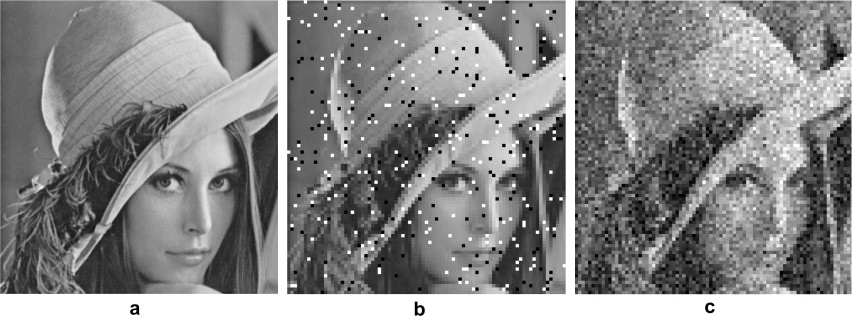
\includegraphics[width=0.9\textwidth]{./imgs/artefatosanalogicos.png}
	\caption{.}
	\label{fig:artefatosanalogicos}
	\fonte{\cite{panagiotopoulou}}
\end{figure}

Em se tratando de vídeos digitais, os artefatos de maior notoriedade são: \emph{blockiness}, \emph{blurriness}, \emph{ringing}, e \emph{noisiness} \cite{farias2007} e podem ser observados na Figura~\ref{fig:artefatosdigitais}, a seguir:

\begin{figure}[!htb]
	\centering
	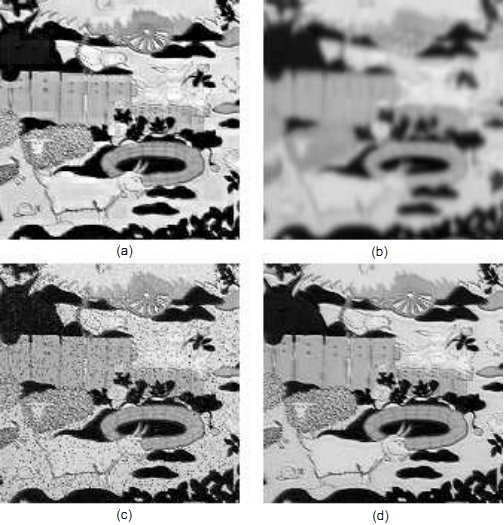
\includegraphics[width=0.9\textwidth]{./imgs/artefatosdigitais.png}
	\caption{.}
	\label{fig:artefatosdigitais}
	\fonte{\cite{farias2007}}
\end{figure}

Poder adicionar artefatos de forma artificial e controlada à vídeos digitais é de grande importância no campo de avaliação de vídeos (tanto na avaliação objetiva quanto na avaliação subjetiva) uma vez que, a partir de algoritmos, é possível simular distorções reais. Estes algoritmos não são padronizados, mas existem algumas recomendações internacionais, como por exemplo a recomendação P.930 da ITU \cite{itup930} que descreve os princípios para reproduzir as distorções relativas à compressão de vídeo sem efetivamente precisar comprimí-lo.

Nas seções que seguem, alguns dos artefatos mais comuns serão detalhados juntamente com as recomendações para a respectiva simulação.

\subsection{Efeito de Blocagem - \emph{Blocking effect}}

Este artefato é o mais estudado pela literatura \cite{emmersonsilva}. Ocorre em função de uma quantização grosseira no processo de compressão, em que resulta numa distorção ou perda de componentes de alta frequência \cite{itup930}. Normalmente ocorre em superfícies lisas em movimento \cite{itup930} \cite{farias2007}.

Muitos codificadores utilizam a Transformada Discreta de Cossenos (DCT - Discrete Cosine Transform), como o MPEG-1 e o MPEG-2, em que uma imagem é codificada a partir de janelas de dimensões 8x8 pixels. 

A recomendação P.930 indica que a simulação deste artefato deve, primeiramente, localizar regiões de movimento em uma imagem para posteriormente selecionar em quais possíveis janelas será aplicada uma média dos valores de luminância \cite{itup930}. Desta forma, o cálculo da DCT e todo o processo de compressão é evitado.

\subsection{Efeito de Borramento - \emph{Blurring effect}}

O artefato de borramento é, visualmente, a perda de nitidez das bordas e de detalhes espaciais em uma imagem, como em áreas com texturas ou ao redor das bordas de objeto de cena \cite{wurao2005}. É causado pelo algoritmo de compressão no momento em que escolhe codificar bits de resolução ou de movimento \cite{itup930}.

A recomendação P.930 fornece os filtros a serem utilizados para a simulação deste artefato.

\subsection{Efeito de Travamento - \emph{Jerkiness}}

Este artefato é facilmente percebido em sistemas com baixa taxa de bits para vídeo, como em sistemas de teleconferência \cite{itup930} em que a imagem parece congelar em determinados instantes. Isso se deve à repetição de \emph{frames} com o objetivo de reduzir a quantidade de informação a ser transmitida ou processada \cite{itup930}.

A recomendação P.930 fornece dois fatores para controlar as repetições numa simulção: o FRF (Frame Repetition Factor) e o EFR (Effective Frame Rate). Um FRF igual a 3 causa a repetição do terceiro \emph{frame} de uma sequência durante os próximos dois \emph{frames}. O EFR é calculado como 30/FRF, e para o exemplo dado tem valor de 10 FPS.

\section{Métricas de Avaliação}

A compressão tende a diminuir a fidelidade, ou seja, o problema da codificação é encontrar um equilíbrio entre o nível de compressão necessário para transmitir pelo canal e o nível de fidelidade que se deseja exibir para o espectador \cite{daronco}.

Apesar de a transmissão digital garantir que a interferência à ruídos seja mínima, a qualidade da imagem não depende somente de interferência, como foi visto. A compressão de vídeos é excelente na perspectiva do transmissor já que o custo do equipamento torna-se menor, porém na perspectiva do receptor/usuário a compressão pode comprometer muito a qualidade.

Neste contexto de tentar equilibrar qualidade e compressão, surge a necessidade de se criarem métodos capazes de avaliar a qualidade dos vídeos transmitidos tanto da parte dos emissores, para saber até que ponto a compressão não é percebida pelo usuário, ou pelo menos que ela não o incomode a ponto de deixar de assistir a transmissão; quanto da parte do usuário, que colabora para ter um serviço melhor.

Diversas metodologias definidas em normas internacionais foram criadas para avaliar a qualidade da informação multimídia (tanto áudio quanto vídeo), divididas em dois paradigmas: avaliação objetiva e avaliação subjetiva, descritas a seguir.

\subsection{Métricas Objetivas}

A avaliação objetiva tenta, através de algoritmos, fazer uma previsão aproximada da qualidade observada pelos observadores \cite{albini}. Os métodos mais simples e mais difundidos são definidos estatisticamente como o MSE (Mean Squared Error - Erro Médio Quadrático) e o PSNR (Peak Signal to Noise Ratio - Razão Sinal-Ruído de Pico) \cite{emmersonsilva} entre os dados originais e os dados recebidos (no caso de vídeos, o cálculo é aplicado pixel a pixel).

Outra métrica objetiva, o SSIM (Structural SIMilarity Index - Indice de Similaridade Estrutural), foi elaborado na tentativa de se aproximar a avaliação às percepções do SVH, pois leva em consideração a luminância, estrutura e o contraste (SILVA). Uma métrica derivada do SSIM é o MSSIM (Mean Structural SIMilarity Index - Indice de Similaridade Estrutural Média), sendo uma média dos valores SSIM calculados a partir do vídeo avaliado (WANG et al, 2004).

\subsubsection{MSE - Mean Squared Error}

O MSE é a média das diferenças ao quadrado entre os valores de nivel de cinza dos pixels. Considerando que o nível de cinza de cada pixel é dado em função de sua posição de acordo com a equação a seguir:

Equação: G = f(t, x, y), onde:

\begin{itemize}
	\item G = nivel de cinza do pixel, dada sua posição;
	\item t = frame onde o pixel está localizado;
	\item x = posição relativa ao eixo vertical no frame;
	\item y = posição relativa ao eixo horizontal no frame.
\end{itemize}

o MSE pode ser calculado conforme a seguinte equação:

    Equação: \[MSE = \frac{1}{\left (T \cdot X \cdot Y \right )} \sum_{t}^{T} \sum_{x}^{X} \sum_{y}^{Y} \left ( P_{1} - P_{2} \right )^{2}\]

para vídeos com T \emph{frames} de tamanho X x Y (WINKLER, 2005).

    Conforme a medida obtida, a seguinte análise é feita: quanto menor o valor do MSE, mais próxima a imagem avaliada está da imagem original \cite{albini}. A imagem da função MSE é o conjunto dos reais, maiores ou iguais a zero, ou seja, um valor zero indica que as imagens são idênticas.

\subsubsection{PSNR - Peak Signal to Noise Ratio}
O PSNR é calculado com base num valor MSE e é dado em escala logarítmica. O PSNR mede a fidelidade entre imagens, ao contrário do MSE que mede diferenças entre imagens (WINKLER, 2005). Esta medida é encontrada conforme a equação a seguir:

Equação: \[PSNR_{dB} = 10 \cdot log_{10} \frac{{\left(2^{n} -1 \right )}^{2}}{MSE}\]

onde n é o número de bits que representa o nível de cinza de cada pixel.

A popularidade na utilização desta métrica se deve ao fato de que o cálculo pode ser realizado rapidamente, sendo bastante utilizado para comparar vídeos comprimidos e descomprimidos (RICHARDSON, 2003; SILVA).

Dentre as limitações desta métrica, está a necessidade de sincronização entre as imagens original e degradada, baixa correlação com as métricas subjetivas definidas na norma ITU-R (ITU-R BT-500.11, Methodology for the Subjective Assessment for the Television Pictures, 2002.; SILVA).

Analisando os resultados, valores de PSNR altos indicam alta fidelidade entre as imagens comparadas, enquanto que valores baixos indicam baixa fidelidade.

\subsubsection{SSIM - Structural Similarity Index}

Esta métrica surgiu com o objetivo de melhor aproximar a avaliação objetiva à percepção humana, pois métricas como o MSE e o PSNR se mostraram ineficientes para tanto \cite{emmersonsilva}. Aplicado sobre valores de luminância, contraste e a estrutura para várias janelas de mesmas dimensões em uma imagem (WANG e BOVIK, 2002), tem como equação:

    Equação: \[SSIM(x, y) = \frac{(2\mu_{x}\mu_{y} + C_{1})(2\sigma_{xy} + C_{2})} {(\mu_{x}^{2} + \mu_{y}^{2}+C_{1})(\sigma_{x}^{2} + \sigma_{y}^{2}+C_{2})}\]

onde:
\begin{itemize}
	\item x e y são janelas sendo comparadas de dimensões NxN;
	\item \(\mu_{x}\) é a média de x;
    \item \(\mu_{y}\) é  a média de y;
    \item \(\sigma^{2}_{x}\) é a variância de x;
    \item \(\sigma^{2}_{y}\) é a variância de y;
    \item \(\sigma_{xy}\) é a covariância de x e y;
    \item C1 = \((k_{1}L)^{2}\), C2 = \((k_{2}L)^{2}\) são duas variáveis para estabilizar a divisão;
    \item L é a faixa dinâmica dos valores dos pixels (normalmente é \(2^{bits por pixel} - 1\));
    \item \(k_{1}\) = 0.01 e \(k_{2}\) = 0.03. Estes são valores são indicados pelos autores do método \cite{wangbovik2004} em decorrência de experimentos realizados.
\end{itemize}

\subsubsection{MSSIM - Mean Structural Similarity Index}

Em termos práticos, normalmente é desejado encontrar-se uma medida de qualidade geral de toda a imagem \cite{wangbovik2004}. Por esta razão, a média dos índices SSIM é calculada:

Equação: \[MSSIM(X, Y) = \frac{1}{M} \sum_{i=1}^{M} SSIM(x_{j}, y_{j})\]

onde:
\begin{itemize}
	\item X e Y são as imagens de referência e distorcida, respectivamente;
	\item \(x_{j}\) e \(y_{j}\) são as janelas dentro das imagens;
	\item M é o número total de janelas na imagem.
\end{itemize}

\subsection{Métricas Subjetivas}

Por causa das limitações das métricas objetivas, muitos trabalhos foram realiz'os nos últimos anos para tentar desenvolver um teste objetivo mais sofisticado que se aproximasse dos resultados subjetivos (WATSON, McGOWAN e MULLIGA, 1999; WANG et al, 2004). Embora muitas métricas tenham sido propostas, nenhuma ofereceu um nível de qualidade em comparação aos testes subjetivos (VQEG, 2003).

A avaliação subjetiva depende de observadores humanos que atribuem notas a partir de suas opiniões sobre a qualidade. Posteriormente, uma análise estatística dos dados coletados é realizada, resultando em uma nota chamada MOS (Mean Opinion Score) \cite{itup930} \cite{albini}. Estes tipos de avaliação possuem algumas recomendações estabelecidas por órgãos internacionais com a finalidade de padronizar os procedimentos e ambientes de avaliação, alguns exemplos destas normas podem ser observados na Tabela \ref{tab:recomendacoes}:

\begin{table}
	\centering
	\caption{Tabela de recomendações da ITU}
	\label{tab:recomendacoes}
	\begin{tabular}{c|l}
		\hline
		\textbf{Nome da Norma} & Descrição \\
		\hline
		\textbf{ITU-R Rec. BT.500} & Metodologias para avaliação subjetiva da qualidade de vídeos \\
			& em televisores \\
		\textbf{ITU-T Rec. P.910} & Métodos para avaliação subjetiva de vídeos em aplicações \\
			& multimídia \\
		\textbf{ITU-T Rec. P.911} & Métodos para avaliação subjetiva de dados audiovisuais em \\
			& aplicações multimídia \\
		\textbf{ITU-T J.144} & Técnicas para avaliação objetiva de vídeo para televisão a cabo na \\
			& na presença de uma referência \\
		\textbf{ITU-R BS.1387} & Avaliação de sistema de áudio de alta qualidade. \\
		\hline
	\end{tabular}
	\fonte{\cite{daronco}}
\end{table}

As metodologias de avaliação seguem diretrizes que dizem respeito aos critérios para escolha das sequências de imagens, à seleção de observadores, a duração das sessões de avaliação, ao tempo de exposição de cada sequência e intervalos de troca, às condições ambiente, etc.

\subsubsection{Método DSIS - Double Stimulus Impairment Scale (Método EBU)}

Comumente usado para avaliação de novos sistemas ou dos prejuízos decorrentes de transmissão. Neste método, ao avaliador é apresentada uma imagem de referência e posteriormente a mesma imagem degradada. As sessões, que devem durar até 30 minutos, podem seguir duas variantes: na primeira, o conjunto referência/degradada é apresentado e ao final o avaliador deve dar uma nota. Na segunda variante, o avaliador é submetido duas vezes ao conjunto referência/degradada e somente ao final lhe é permitido dar a nota. Em ambas a apresentação dos conjuntos referência/degradada é aleatória.

A Figura \ref{fig:dsisvariantes} apresenta as fases de apresentação para cada variante. Em T1 e T3 o avaliador deve observar as imagens. O período T2 é de transição, deve ser apresentada uma tela cinza por 3 segundos. Por fim, o período T4 é o de avaliação, onde o avaliador efetivamente pode dar a nota. A Tabela \ref{tab:dsisfases} sintetiza as fases e os períodos recomendados.

\begin{figure}[!htb]
	\centering
	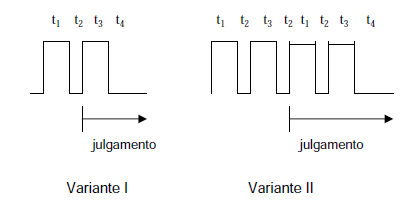
\includegraphics[width=0.9\textwidth]{./imgs/dsisvariantes.png}
	\caption{.}
	\label{fig:dsisvariantes}
	\fonte{Fonte: ITU-R BT.500-11.}
\end{figure}

\begin{table}
	\centering
	\caption{Fases DSIS}
	\label{tab:dsisfases}
	\begin{tabular}{c|l}
		\hline
		\textbf{T1 = 10 s} & Imagem de referência \\
		\textbf{T2 = 3 s} & Cinza intermediário, nível de vídeo 200mV \\
		\textbf{T3 = 10 s} & Imagem degradada \\
		\textbf{T4 = 5-11 s} & Cinza intermediário \\
		\hline
	\end{tabular}
	\fonte{Fonte: ITU-R BT.500-11.}
\end{table}

A escala de avaliação a ser utilizada é dada conforme a Tabela \ref{tab:dsisescala}.

\begin{table}
	\centering
	\caption{Escala de avaliação DSIS}
	\label{tab:dsisescala}
	\begin{tabular}{c|l}
		\hline
		\textbf{5} & Imperceptível \\
		\textbf{4} & Perceptível, mas não irritante \\
		\textbf{3} & Pouco incômoda \\
		\textbf{2} & Irritante \\
		\textbf{1} & Bastante Irritante \\
		\hline
	\end{tabular}
	\fonte{Fonte: ITU-R BT.500-11.}
\end{table}

\subsubsection{Método DSCQS - Double Stimiulus Continuous Quality Scale}

Este método também é aplicável para avaliar os efeitos dos meios de transmissão sobre a qualidade da imagem. Assim como no método DSIS, as imagens são apresentadas aos pares. Uma deve ser a imagem original e a outra deve ser a imagem processada pelo sistema em teste. A ordem de qual será apresentada por primeiro, bem como a ordem de apresentação de cada par, é aleatória. Outra diferença do método DSIS está na avaliação: o avaliador deve dar nota para ambas as imagens.

O número de repetições dos vídeos depende da duração da sequência de teste. Cenas mais estáticas devem durar de 3 a 4 segundos, podendo ser repetidas 5 vezes (as duas últimas são avaliadas), já cenas mais dinâmicas, que possuam artefatos variantes no tempo, devem durar 10 segundos e ser repetidas duas vezes (a segunda é avaliada).

As fases da apresentação DSCQS podem ser observadas na Figura \ref{fig:dscqsfases}. Elas são semelhantes as fases do método DSIS, a diferença está no momento em que a avaliação é permitida. 

\begin{figure}[!htb]
	\centering
	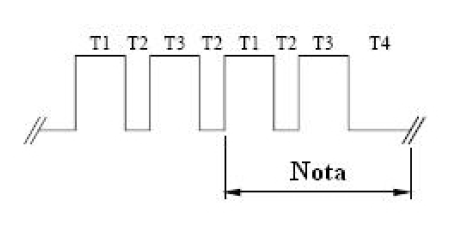
\includegraphics[width=0.9\textwidth]{./imgs/dscqsfases.png}
	\caption{.}
	\label{fig:dscqsfases}
	\fonte{Fonte: ITU-R BT.500-11.}
\end{figure}

\begin{table}
	\centering
	\caption{Fases DSCQS}
	\label{tab:dsisfases}
	\begin{tabular}{c|l}
		\hline
		\textbf{T1 = 10 s} & Vídeo de teste A \\
		\textbf{T2 = 3 s} & Cinza intermediário, nível de vídeo 200mV \\
		\textbf{T3 = 10 s} & Vídeo de teste B \\
		\textbf{T4 = 5-11 s} & Cinza intermediário \\
		\hline
	\end{tabular}
	\fonte{Fonte: ITU-R BT.500-11.}
\end{table}

Para realizar a avaliação, o avaliador deve marcar as notas em uma escala contínua conforme a apresentada na Figura \ref{fig:dscqsescala}.

\begin{figure}[!htb]
	\centering
	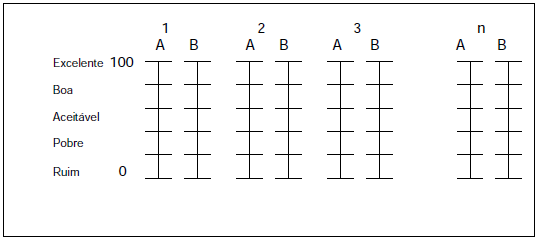
\includegraphics[width=0.9\textwidth]{./imgs/dscqsescala.png}
	\caption{.}
	\label{fig:dscqsescala}
	\fonte{Fonte: ITU-R BT.500-11.}
\end{figure}

\subsubsection{Método SSCQE - Single Stimulus Continuous Quality Evaluation}

Neste método, uma série de segmentos de programa são apresentados ao grupo de avaliadores com duração mínima de cinco minutos. Assim como no método DSCQS, a escala de avaliação é contínua. Os avaliadores modificam a nota conforme desejarem ao longo da apresentação das sequências. As notas, que são amostradas duas vezes por segundo, permitem o levantamento de histogramas (Fonte: REHME).

Este método é mais adequado para avaliar a qualidade de vídeo em sequências longas e sem referência, o que é mais próximo da realidade.

\subsubsection{Método SDSCE - Simultaneous Double Stimulus for Continuous Evaluation Method}

Para este método, as sequências de referência e de teste são apresentadas de forma simultânea. O avaliador deve julgar a fidelidade do vídeo em teste utilizando a escala contínua, assim como nos métodos DSCQS e SSCQE. A Figura \ref{fig:sdsce} demonstra como deve ser realizada a apresentação.

\begin{figure}[!htb]
	\centering
	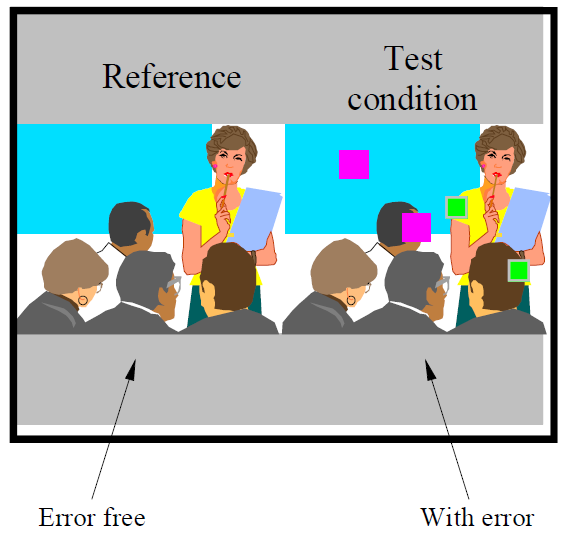
\includegraphics[width=0.9\textwidth]{./imgs/sdsce.png}
	\caption{.}
	\label{fig:sdsce}
	\fonte{Fonte: ITU-R BT.500-11.}
\end{figure}

As sequências podem ser apresentadas lado a lado no mesmo monitor ou em monitores diferentes, desde que tenham as mesmas especificações e características.

\section{Distribuições de Probabilidade}

Distribuição de probabilidade é um conceito fundamental em Estatística, utilizado em nível prático e teórico \cite{distteoria}.

As distribuições de probabilidade são funções matemáticas que mapeiam para todo valor dentro de um intervalo definido (discreto ou contínuo), valores de probabilidade de ocorrência, considerando uma variável aleatória que pode assumir qualquer valor deste intervalo\cite{distteoria}. Em outras palavras, é a função que descreve a probabilidade de uma variável aleatória assumir determinados valores \cite{wikidistribuicoes}.
 
Distribuições discretas são funções de probabilidade cuja variável pode assumir um número discreto de valores, não necessariamente finito. A definição matemática de uma função de probabilidade discreta, p(x), é uma função que satisfaz as seguintes propriedades:

\begin{itemize}
	\item A probabilidade de x assumir um valor específico é p(x);
	\item p(x) é não negativa para todo x real;
	\item a soma de p(x) para todos os valores possíveis de x é igual a 1.
\end{itemize}

Distribuições contínuas ou funções de probabilidade contínua são definidas para infinitos valores dentro de um intervalo. Por este fato, a probabilidade é medida para subintervalos, uma vez que a probabilidade de qualquer ponto é sempre zero\cite{distteoria}.

A definição matemática de uma função de probabilidade contínua, f(x), é uma função que satisfaz as seguintes propriedades:

\begin{itemize}
	\item a probabilidade de x estar entre dois pontos a e b é: \(p[a \leqslant x \leqslant b] = \int_{a}^{b}f(x)dx\);
	\item a probabilidade é sempre não-negativa para todo x real;
	\item a integral da função de probabilidade é: \(\int_{-\infty}^{\infty}f(x)dx = 1\)
\end{itemize}

Normalmente, distribuições de probabilidade são definidas por suas funções densidade de probabilidade, que associam a cada valor de x, sua probabilidade de ocorrência, de acordo com a equação a seguir: 

Equação: \(f(x) = Pr[X = x]\).

Particularmente para distribuições contínuas, a densidade de probabilidade é definida como a integral entre dois pontos, já que para qualquer ponto a probabilidade deve ser zero, como já descrito:

Equação: \(\int_{a}^{b}f(x)dx = Pr[a \leqslant X \leqslant b]\).

Algumas distribuições de probabilidade bastante conhecidas, como por exemplo a distribuição normal e a uniforme, são detalhadas a seguir.

\subsection{Distribuição Uniforme}

Distribuição uniforme contínua, ou distribuição retangular, é aquela em que todos os intervalos de mesmo tamanho tem a mesma probabilidade de ocorrer \cite{wikidistuniform1}. Mais precisamente, a probabilidade de se gerar qualquer ponto em um intervalo contindo no espaço amostral é proporcional ao tamanho do intervalo \cite{wikidistuniform2}. Em uma distribuição uniforme discreta, para todos os elementos possíveis a probabilidade é a mesma.

A equação da função densidade de probabilidade contínua dada a seguir, é exemplificada na Figura \ref{fig:uniformdist}.

Equação: \[\left\{\begin{matrix}
\frac{1}{(b-a)} & \mbox{para } a \leqslant x \leqslant b,\\ 
0 & \mbox{para } x < a \mbox{ ou } x > b
\end{matrix}\right.\]

\begin{figure}[!htb]
	\centering
	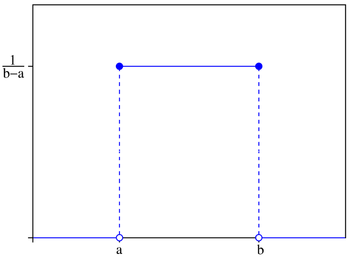
\includegraphics[width=0.9\textwidth]{./imgs/uniformdist.png}
	\caption{Função Densidade de Probabilidade de Distribuição Uniforme.}
	\label{fig:uniformdist}
	\fonte{\cite{wikidistuniform1}}
\end{figure}

Uma distribuição uniforme que seja definida dentro do intervalo (0, 1) é chamada de Distribuição Uniforme Padrão (U(0, 1)). A partir dela é possível gerar distribuições em diferentes intervalos (a, b) conforme a equação a seguir:

Equação: \[a+[(b-a) \cdot U(0, 1)]\]

Muitas linguagens de programação, assim como Java e C++, possuem funções nativas para gerar valores uniformemente distribuídos. Em Java, a classe Math possui a função random() que gera valores de acordo com uma distribuição uniforme padrão. Ainda, Java possui uma classe especializada no pacote util chamada Random, utilizada para gerar valores booleanos, de \emph{bytes}, de pontos flutuantes, etc. Esta classe também gera valores seguindo uma distribuição normal através do método nextGaussian(), que utiliza a transformada Box-Mueller, explicada na próxima seção \cite{javaapi}. 

Na linguagem C++ a função rand() encontra-se na biblioteca padrão (cstdlib ou stdlib.h), assim como a função srand() que inicializa a semente do gerador. O gerador, ao contrário de Java, fornece valores inteiros no intervalo (0, RAND\_MAX). A constante RAND\_MAX, também da biblioteca padrão, tem valor 32767 \cite{cppreference}.

\subsection{Distribuição Normal}

Conhecida também como Função Gaussiana, esta distribuição de probabilidade tem domínio nos reais no intervalo \((-\infty, \infty)\). É definida de acordo com dois parâmetros: a média \((\mu)\), ou valor esperado, e a variância \((\sigma^{2})\), conforme a seguinte equação:

Equação: \(f(x; \mu, \sigma^2) = \frac{1}{\sigma\sqrt{2\pi}}e^{-\frac{1}{2}(\frac{x - \mu}{\sigma})^2}\).

onde:
\begin{itemize}
	\item \(f(x; \mu, \sigma^2)\) é a probabilidade de ocorrência do valor x;
	\item \(\mu\) é o valor da média;
	\item \(\sigma\) e \(\sigma^{2}\) são os valores desvio padrão e variância, respectivamente.
\end{itemize}

A Figura \ref{fig:normaldist} apresenta diferentes funções densidade de probabilidade normal para diferentes parâmetros de média e variância.

\begin{figure}[!htb]
	\centering
	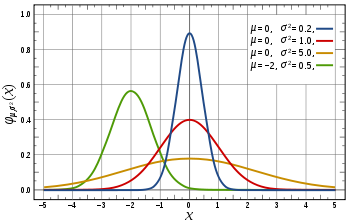
\includegraphics[width=0.9\textwidth]{./imgs/normaldist.png}
	\caption{Função Densidade de Probabilidade de Distribuição Normal.}
	\label{fig:normaldist}
	\fonte{Fonte: \cite{wikinormaldist}}
\end{figure}

Na Teoria das Probabilidades, o Teorema do Limite Central afirma que, dada certas condições, a média de um número suficientemente grande de variáveis aleatórias independentes, cada uma com média e variância finita, seguirá uma distribuição normal \cite{teoremalimitecentral}.

Em teoria, uma variável aleatória seguindo uma distribuição normal pode assumir valores infinitos, o que é inconveniente computacionalmente. Desta forma, é bastante comum aplicar-se o truncamento desta distribuição, em que um limite inferior e/ou superior é utilizado para adequar os resultado a um intervalo desejado.

Existem algumas formas de se construir computacionalmente um gerador aleatório que segue uma distribuição normal. Dois métodos bastante conhecidos são: transformada de Box-Mueller e algoritmo de Ziggurat.

A transformada de Box-Mueller se baseia num gerador aleatório com distribuição uniforme pode ser expresso em duas formas: a básica e a polar. Na primeira, o gerador uniforme deve gerar valores no intervalo (0, 1], na segunda forma devem ser gerados valores no intervalo [-1, +1] como valores de entrada \cite{boxmueller}.

Supondo que \(U_{1}\) e \(U{2}\) são variáveis aleatórias com distribuição uniforme no intervalo (0, 1] (ou seja, forma básica), as variáveis \(Z_{0}\) e \(Z_{1}\), dadas conforme as equações a seguir, seguirão uma distribuição normal com desvio padrão igual a 1.

Equações:
\[Z_{0} = R\cos{(\Theta)} = \sqrt{-2\ln{U_{1}}}\cos{(2\pi U_{2})}\]
\[Z_{1} = R\sin{(\Theta)} = \sqrt{-2\ln{U_{1}}}\sin{(2\pi U_{2})}\]

A forma polar da transformada pode ser calculada conforme as equações a seguir. Nesta forma, a vantagem reside no fato de que as funções trigonométricas não precisam ser calculadas diretamente \cite{wikiboxmueller}. Considerando que u e v são variáveis uniformemente distribuídas,  e \(s = u^{2} + v^{2}\), as variáveis \(z_{0}\) e \(z{1}\) seguirão uma distribuição normal:

\[z_{0} = \sqrt{-2\ln{U_{1}}}\cos{(2\pi U_{2})} = \sqrt{-2\ln{s}}(\frac{u}{\sqrt{s}})\cos{(2\pi U_{2})}) = u\sqrt{\frac{-2\ln{s}}{s}}\]
\[z_{1} = \sqrt{-2\ln{U_{1}}}\sin{(2\pi U_{2})} = \sqrt{-2\ln{s}}(\frac{v}{\sqrt{s}})\cos{(2\pi U_{2})}) = v\sqrt{\frac{-2\ln{s}}{s}}\]

As condições de validade são: garantir que s seja maior que zero e menor que um. Caso alguma destas condições seja violada, deve-se gerar novos valores de u e v até que as condições sejam satisfeitas.

O Algoritmo Ziggurat se baseia, assim como a transformada Box-Mueller em sua forma polar, no algoritmo de rejeição para gerar valores. Normalmente é utilizado quando a geração de uma grande quantidade de números é necessária \cite{ziggurat}. 

\subsection{Distribuição Triangular}

Esta distribuição, como o nome diz, tem formato triangular. Sua função densidade de probabilidade varia de acordo com três parâmetros: a, b e c, como pode ser observado nas equações a seguir e na Figura \ref{fig:triangulardist}.

\[\left\{\begin{array}{l l}
0 & \mbox{para } x < a \\ 
\frac{2(x-a)}{(b-a)(c-a)} & \mbox{para } a \leqslant x \leqslant c, \\
\frac{2(b-x)}{(b-a)(b-c)} & \mbox{para } c \leqslant x \leqslant b, \\
0 & \mbox{para } b < x
\end{array}\right.\]

\begin{figure}[!htb]
	\centering
	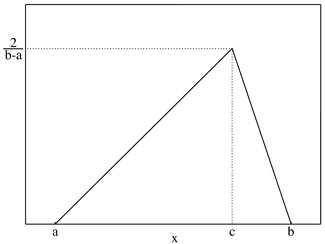
\includegraphics[width=0.9\textwidth]{./imgs/triangulardist.png}
	\caption{Função Densidade de Probabilidade de Distribuição Triangular.}
	\label{fig:triangulardist}
	\fonte{\cite{wikitriangulardist}}
\end{figure}

Computacionalmente é possível criar um gerador aleatório que segue esta distribuição a partir de um gerador aleatório que siga uma distribuição uniforme no intervalo (0, 1) através das equações a seguir:

\[\left\{\begin{array}{l l}
X = a +\sqrt{U(b-a)(c-a)} & \mbox{para } 0 < F(c)\\ 
X = b - \sqrt{(1-U)(b-a)(b-c)} & \mbox{para } F(c) \leqslant U < 1
\end{array}\right.\]

\section{Trabalhos Relacionados}

\section{Resumo e Conclusão do Capítulo}


Comparando-se as metodologias, ambas são importantes e ambas têm suas limitações. A avaliação objetiva é mais precisa considerando que ela avalie a diferença entre um vídeo original e o efetivamente observado. Porém, nem sempre o vídeo original possui uma qualidade que satisfaria o telespectador, sendo esta, portanto, uma de suas desvantagens.

A avaliação subjetiva embora seja um processo mais difícil de ser realizado por depender de um grande grupo de pessoas e tenha um custo mais elevado \cite{albini}, segundo \cite{wangbovik2004} esta é o tipo de avaliação mais ‘correta’, pois o próprio telespectador realiza a avaliação.


%----------- Terceiro Capítulo: Metodologia --------------

\chapter{Especificação} %(ou especifiação) 10 --- 20 pags

O \emph{software} a ser desenvolvido neste trabalho deverá fornecer uma ferramenta flexível de degradação de vídeo digital e também de avaliação subjetiva e objetiva das mídias.
Neste capítulo serão apresentados os requisitos de tal sistema, assim como as especificações de desenvolvimento, arquitetura e funcionamento.

\section{Análise de Requisitos}

A análise de requisitos é parte fundamental de qualquer projeto, buscando atender da melhor forma as necessidades dos futuros usuários.
Esta sessão descreve os requisitos levantados durante o estudo e planejamento da ferramenta.

\subsection{Requisitos Funcionais}

Requisitos funcionais são aqueles determinados pelas funcionalidades exigidas do sistema, ou seja, as ações que se espera que o sistema execute. 
Foram levantados os seguintes requisitos funcionais:

\begin{itemize}
	\item O \emph{software} deverá possuir ferramentas de degradação de vídeos digitais de blocagem e borramento.
	\item O \emph{software} deverá possuir uma ferramenta de simulação de transmissão \emph{streaming}.
	\item O \emph{software} deverá ser capaz de criar e gerenciar sessões de avaliação subjetiva.
	\item O \emph{software} deverá possuir uma ferramenta que realize avaliação objetiva sobre os vídeos da base de dados, conforme as métricas PSNR, MSE e MSSIM.
	\item O \emph{software} deverá ser capaz de exibir os vídeos existentes na base de dados.
	\item O \emph{software} deverá exibir os resultados das avaliações objetivas e subjetivas de forma gráfica.
\end{itemize}

\subsection{Requisitos Não-Funcionais}

Requisitos não-funcionais são aqueles ditados por restrições ou exigências de qualidade ou de operação, tais como performance, segurança ou tecnologias envolvidas.
Abaixo se encontram os requisitos não funcionais levantados:

% TODO dividir por categorias: padronização, usabilidade, tecnologias envolvidas.

\begin{itemize}
	\item As ferramentas de degradação e métricas objetivas deverão operar sobre vídeos em formato YUV planificado com subamostragem 4:2:0.
	\item A ferramenta de simulação deverá operar sobre vídeos no formato \sigla{H.262}{Padrão de compressão de vídeo digital também conhecido MPEG-2 Part 2} encapsulados em um Transport Stream (\sigla{TS}{Transport Stream}).
	\item O sistema deve fornecer documentação detalhada de auxílio ao uso das ferramentas.
	\item A ferramenta de exibição deverá ser executada em um sistema capaz de prover um \emph{display} com resolução igual ou maior que a dos vídeos a serem exibidos.
	% TODO verificar a versão da JRE necessária para rodar a interface
	\item A interface gráfica do sistema necessita que haja um \emph{Java Runtime Environment} (\sigla{JRE}{Java Runtime Environment}) instalado no sistema operacional.
	\item O \emph{player} de vídeo MPlayer, livre e de código aberto, é necessário para mostrar os vídeos durante as sessões.
\end{itemize}

\section{Especificações do Software}

Esta seção tem o propósito de descrever a arquitetura proposta para o SASQV2, assim como abordar as diferentes linguagens e bibliotecas que ajudam a integrar o programa.

\subsection{Arquitetura do Sistema}

Por se tratar da continuação do desenvolvimento do projeto SASQV, este trabalho reutiliza e adapta grande parte dos componentes existentes no trabalho original.

A Figura \ref{fig:arquitetura} mostra uma comparação entre as visões gerais de ambos os projetos. A diferença mais notável entre estas arquiteturas é a separação dos componentes de serviço e o de ferramentas, além de também recriar o componente de interface gráfica para melhor atender às necessidades do sistema.

Mais detalhes sobre cada componente da arquitetura são descritos em seções específicas a seguir.

\begin{figure}[!htb]
	\centering
	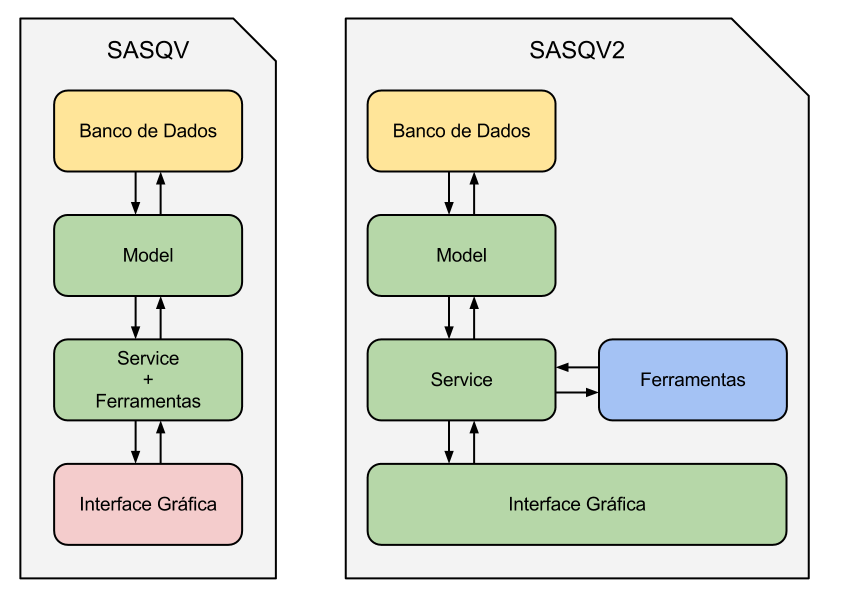
\includegraphics[width=0.9\textwidth]{./imgs/arquitetura.png}
	\caption{Visão geral das arquiteturas dos sistemas SASQV e SASQV2.}
	\label{fig:arquitetura}
	\fonte{Autoria Própria.}
\end{figure}

\subsubsection{Banco de Dados}

O componente banco de dados foi completamente reaproveitado, seguindo as mesma especificações do SASQV.

O Sistema Gerenciador de Banco de Dados (\sigla{SGBD}{Sistema Gerenciador de Banco de Dados}) escolhido foi o MySQL, atualmente o SGDB \emph{open source} mais utilizado no mundo \cite{mysqlmarket}.
O MySQL foi lançado e desenvolvido em 1995 pela empresa Sueca MySQL AB, atualmente incorporada pela Oracle Corporation, na forma de um SGDB que fornece um servidor multi-usuários para bancos de dados relacionais \cite{wikipediamysql}.

Juntamente do MySQL também é utilizado o MySQL Workbench, uma ferramenta distribuída pela Oracle que concilia um cliente MySQL, uma ferramenta de \emph{Database Moddeling} e um administrador de servidor MySQL.

A versão \emph{open source} de ambas as ferramentas é distribuída sob a licensa GNU General Public License (\sigla{GPL}{General Public License}).

O modelo Entidade-Relacionamento (\sigla{ER}{Entidade-Relacionamento}) é o mesmo utilizado pelo SASQV, como mostrado na Figura \ref{fig:diagramaER}.

\begin{figure}[!htb]
	\centering
	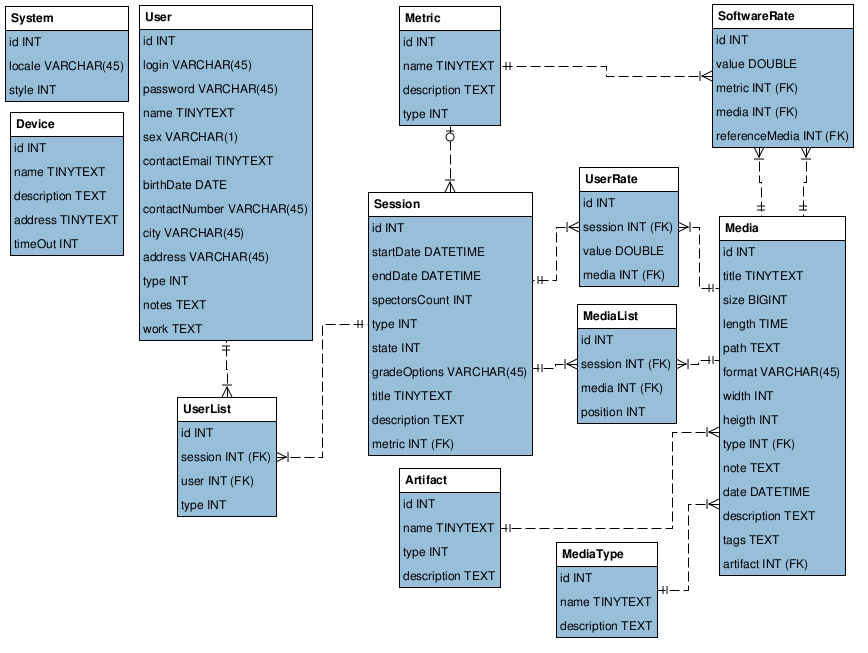
\includegraphics[width=0.9\textwidth]{./imgs/diagramaER.png}
	\caption{Diagrama Entidade-Relacionamento do SASQV2}
	\label{fig:diagramaER}
	\fonte{Autoria Própria}
\end{figure}

\subsubsection{Model}

O componente Model presente no SASQV2 também foi inteiramente reaproveitado do SASQV, cabendo apenas algumas adições. Este componente consiste na implementação de um mapeamento objeto-relacional (\sigla{MOR}{Mapeamento Objeto Relacional}) por meio da biblioteca Hibernate.

O Hibernate teve seu desenvolvimento iniciado em 2001 por Gavin King, com o objetivo de melhorar as ferramentas de persistência existentes na plataforma Java \cite{hibernateHistory}, e é atualmente distribuído sob a licensa GNU Lesser General Public License (\sigla{LGPL}{Lesser General Public License}) \cite{hibernateAbout}.

A biblioteca provê um mapeamento flexível entre objetos Java e tipos SQL, eliminando a custosa necessidade de processamento manual e repetitivo de listas de resultados obtidas via SQL e JDBC.
Estima-se que até cerca de 30\% do código de uma aplicação possa ser poupado utilizando MOR, além de incrementar a portabilidade do sistema suportando diversas implementações de Bancos de Dados SQL em troca de um pequeno \emph{overhead} de performance.

\subsubsection{Service}

Este elemento também foi reaproveitado, no entanto sofreu diversas adaptações em sua estrutura para comportar novas funcionalidades e continuar suportando as antigas.
O componente presente no SASQV se trata de uma fachada de serviço responsável por interpretar mensagens provenientes da interface e distribuí-las em uma das três formas a seguir:

\begin{enumerate}
	\item Executar uma ação de degradação ou métrica objetiva.
	\item Repassar uma ação para o dispositivo sem-fio e esperar por resposta.
	\item Repassar uma ação para o elemento model e esperar por resposta.
\end{enumerate}

Na arquitetura do SASQV2 a interpretação de mensagens foi descartada, uma vez que foi prosposta a implementação de uma nova interface em linguagem Java, que deu lugar a métodos de finalidades distintas dentro de cada ação enumerada acima. % TODO verificar se o acima pode virar abaixo?!!?
Com isso a execução de tarefas de degradação ou avaliação por métrica objetiva, antes executadas localmente, passaram a ser delegadas para um novo componente chamado Ferramentas, descrito em \ref{met:ferramentas}.

Já o conteúdo dos métodos que repassam as ações para o dispositivo sem-fio e para o model permanecem muito semelhantes aos encontrados na interpretação de mensagens originalmente feito no SASQV, sofrendo apenas pequenas modificações para acomodar a nova estrutura.

\subsubsection{Ferramentas}
\label{met:ferramentas}

O módulo ferramentas constitui um novo componente na arquitetura do \emph{software}, visto que um dos objetivos deste trabalho é desenvolver melhores ferramentas de degradação considerou-se válida a separação deste módulo que originalmente se encontrava juntamente do Service.

Esse módulo é resposável por todas as ferramentas que de alguma forma manipulam vídeos digitais ou auxilíam nesta manipulação. Dessa forma foram desenvolvidas 5 ferramentas distintas, em linguagem C++:

\begin{description}
	\item[Block] Cria o efeito de blocagem nos vídeos.
	\item[Blur] Cria o efeito de embaçamento nos vídeos.
	\item[Netsim] Efetua uma simulação de streaming de vídeo digital com perda informação.
	\item[Raffle] Ferramenta auxíliar para distribuição temporal e espacial dos artefatos.
	\item[Metric] Efetua avaliação dos vídeos por meio de métricas objetivas.
\end{description}

Estas ferramentas podem receber configurações independentes e flexíveis, diversificando as possibilidades de geração de degradações e artefatos e tornando possível a criação de resultados diferenciados para um mesmo vídeo usado como referência. Dentre essas configurações pode-se destacar a distribuição dos artefatos no tempo e no espaço e a intensidade de aplicação dos mesmos. Cada ferramenta citada será descrita com mais detalhes em \ref{des:ferramentas}. 

\subsubsection{Interface Gráfica}


Originalmente desenvolvida utilizando a tecnologia Adobe Flex, era necessária a utilização de uma biblioteca exclusivamente para comunicação entre os módulos de Interface e Service. A biblioteca utilizada (merapi) se encontrava em fase de desenvolvimento beta e carecia de funcionalidades, de forma que seria necessário buscar uma biblioteca alternativa para continuar o densevolvimento do projeto.

Além disso, as ferramentas de desenvolvimento em tecnologia Flex não são gratuitas e perderam gradativamente o suporte à sistemas operacionais Linux.

A combinação destes fatores motivou a decisão de desenvolver uma nova intercae Gráfica utilizando Java, proporcionando melhor integração, reduzindo o envolvimento de diversas tecnologias e bibliotecas e assim aumentando a portabilidade da ferramenta.

\subsection{Linguagens}

Por se tratar da aprimoração e continuação do projeto SASQV a primeira linguagem contemplada foi a presente no mesmo: Java.

Esta foi desenvolvida por uma equipe de programadores liderada por James Gosling, trabalhando para a empresa Sun MicroSystems \cite{wikijava}. Sendo lançada em 1995, era o principal componente da plataforma Java e demonstrava forte inspiração na linguagem C++, compartilhando parte de sua sintaxe e também diversas característica.

No entanto, Java é considerada uma linguagem de mais alto nível, além de ser compilada no formato \emph{bytecode}, o que favorece a portabilidade dos programas, podendo ser executados em diversas arquiteturas e sistemas operacionais, contanto que estes possuam uma implementação da Java Virtual Machine (\sigla{JVM}{Java Virtual Machine}). Uma das facilidades da linguagem é a sua extensa biblioteca padrão, que contém, entre outros, diversos componentes para construção de interfaces gráficas.

A linguagem C++ também passou a ser considerada para o desenvolvimento do projeto, visto o desenvolvimento do módulo de Ferramentas como programas que possam ser usados independentemente.
A linguagem teve seu desenvolvimento iniciado por Bjarne Stroustrup em 1979, quando trabalhava na Bell Labs \cite{wikicplusplus}.
C++ é uma nova implementação da linguagem C adicionada de novas funcionalidades, tais como suporte a classes, sobrecarga de operadores, herança múltipla e tratamento de exceções.
Atualmente, C++ é uma das linguagens mais populares, sendo implementada em diversas plataformas de \emph{hardware} e sistemas operacionais, além de ser usada na implemantação dos mais diversos \emph{softwares} para \emph{desktop}, \emph{drivers} de dispositivos de \emph{hardware} e sistemas embarcados.

Um dos principais atrativos da linguagem para o desenvolvimento das ferramentas deste projeto é a existência de diversas funcionalidades de baixo nível.
Essas funcionalidades simplificam e facilitam o acesso e manipulação \emph{byte} a \emph{byte} de \emph{streams} de dados, algo que é usado extensivamente ao longo da implementação das ferramentas.
Outro aspecto importante derivado destas funcionalidades é o impacto na performance do software. 
Segundo \cite{benchmarks}, para o \emph{benchmark reverse-complement} --- onde são efetuadas diversas operações de leitura e escrita em arquivos, além de um leve processamento --- a melhor implementação em Java foi 1.9 vezes mais lenta que a melhor implementação em C++.
A simplicidade da linguagem também facilita o desenvolvimento de ferramentas \emph{stand-alone} com interface por linhas de comando, além de possuir diversas bibliotecas de \emph{parsing} para comandos e opções.

Ambas as linguagens eram previamente conhecidas pelos integrantes do projeto, os quais também possuem um nível confortável de experiência no desenvolvimento de aplicações com estas linguagems e com diversas ferramentas associadas a elas, como IDE's, bibliotecas gráficas e conectividade com bancos de dados.

\subsection{Bibliotecas}
\subsection{Diagramas de Caso de Uso}
\section{Considerações}

Para este projeto de \emph{software} procurou-se aproveitar ao máximo os componentes existentes no SASQV, de forma a maximizar o esforço nos aspectos a serem melhorados e não consumir tempo de projeto retrabalando o que já foi feito. 

A adesão ao desenho de \emph{software} apresentado se justifica pela independência entre os componentes, facilitando o desenvolvimento e teste de cada um e também o reaproveitamento em trabalhos futuros.
A opção por criar ferramentas independentes para o processo de degradação se mostra eficiente e versátil, visto que deste modo estão prontas para serem reutilizadas e combinadas à outras ferramentas, além de facilitarem a automatização do processo de degradação para o usuário avançado.

Sendo assim, a estrutura planejada foi muito semelhante à do projeto original, com diversos componentes sofrendo adaptações e também a adição de um novo componente dedicado.


%---------- Quarto Capítulo: Desenvolvimento ----------

\chapter{Desenvolvimento} %10 --- 20 pags

Este capítulo descreve como efetivamente foi realizado o projeto, forma de trabalho, ferramentas utilizadas, resultados obtidos (ferramentas e \emph{interfaces}), ou seja, o reflexo das decisões de projeto tomadas que foram abordadas no capítulo anterior.

\section{Ferramentas Utilizadas}
\subsection{Sistema Operacional}

O desenvolvimento deste projeto foi totalmente realizado em ambiente Linux, em diferentes distribuições derivadas do Debian: Ubuntu 12.04 e Xubuntu 11.10.

\subsection{Ambientes de Desenvolvimento Integrado}

A primeira etapa de desenvolvimento planejada foi a de construir um modelo para a nova \emph{interface} gráfica. Tendo em vista a linguagem Java como requisito, optou-se pelo \sigla{IDE}{Integrated Development Environment} NetBeans (versão 7.1.1) que possui uma ferramenta nativa específica para a construção de \emph{interfaces} gráficas para usuário, a \sigla{GUI}{Graphical User Interface} Builder (\emph{Graphical User Interface}). Esta ferramenta permite a construção de formulários no estilo drag-and-drop de containers existentes no Java, como por exemplo JFrame, JPanel, JButton, etc.

Inicialmente, o IDE Eclipse também foi utilizado com a finalidade de se realizar modificações nos projetos originais model e service. Posteriormente, para unificar o projeto em apenas um ambiente de desenvolvimento, os projetos originais foram importados no NetBeans.

\subsection{Outras ferramentas}

Os códigos em C++ foram desenvolvidos através do editor de textos Vim, um editor de textos gratuito e de código aberto amplamente configurável para permitir edições eficientes de texto \cite{vimabout}. Este editor é uma versão aperfeiçoada do editor Vi, presente na maioria dos sistemas \sigla{UNIX}{Sistema Operacional}.

Para criar executáveis dos códigos C++ gerados, foi utilizado o compilador g++. Este compilador faz parte da coleção de compiladores \sigla{GCC}{GNU Compiler Collection} \cite{gccabout} produzida e mantida pelo GNU \emph{Project} \cite{gnuabout}.

A fim de automatizar o processo de geração de executáveis, a ferramenta \emph{make} foi configurada de acordo. Esta ferramenta, também mantida pelo GNU Project, permite que vários códigos-fonte sejam processados ao mesmo tempo através de um arquivo de configuração chamado \emph{makefile}, que pode executar um compilador para gerar arquivos-objeto, ou executar um \emph{linker} para gerar executáveis \cite{makeabout}.
 
\subsection{Controle de Versões}

Em função de a equipe contar com dois integrantes desenvolvedores, existe a necessidade de se utilizar uma ferramenta para o controle de versões do projeto. Primeiramente, para realizar testes de algumas funcionalidades foi preciso modificar radicalmente o código o que, em certos casos, não gerou resultados satisfatórios, sendo necessário retornar à um ponto estável e funcional. Além deste motivo, o sistema de controle de versões escolhido, o Git, possui ferramentas de resolução de conflitos eficientes que auxiliam o desenvolvimento simultâneo.

O Git é um software livre e gratuito distribuído sob a licença \sigla{GNU}{Projeto de desenvolvimento de software livre} General Public License versão 2 \cite{git}.

Aliado a esta ferramenta, foi utilizado um serviço web de hospedagem de projetos que é organizado pelo sistema de controle de versões Git, o GitHub cujo endereço é http://github.com. Existem funcionalidades no estilo rede social como feeds, seguidores e gráficos diversos, bem como funcionalidades de projeto como visualização de pastas e códigos, gráficos de desempenho por usuário, por equipe, por período de desenvolvimento, frequência de código, histórico de modificações, entre outros \cite{githubabout}.

Na versão gratuita, que foi a utilizada, há uma exigência: que o código seja aberto \cite{githubabout}. Na versão paga, existem planos que permitem a criação de repositórios privados com times de desenvolvimento. Para ambas as versões o número de colaboradores é ilimitado, assim como o número de repositórios públicos.

\section{Ferramentas Desenvolvidas}
\label{des:ferramentas}

As ferramentas foram planejadas para uma utilização modular, ou seja, para serem utilizadas através da \emph{interface} do SASQV assim como através da linha de comando, de forma independente. Um dos requisitos destas ferramentas é a de que sejam aplicadas sobre vídeos no formato YUV com subamostragem 4:2:0 \emph{progressive}.

\subsection{Raffle}
\label{des:raffle}

A ferramenta \emph{raffle} tem como objetivo gerar elementos aleatórios multi-dimensionais no domínio dos naturais, armazenado-os em arquivo.

No arquivo gerado, cada coluna representa uma dimensão que deve seguir alguma distribuição de probabilidade, informada via parâmetros. Dentre as distribuições possíveis e seus respectivos parâmetros tem-se: 

\begin{itemize}
	\item Distribuição constante: a dimensão correspondente terá valor constante c para todos os elementos gerados.
	\item Distribuição uniforme: a dimensão correspondente terá valores uniformemente gerados num intervalo [a, b).
	\item Distribuição normal: a dimensão correspondente terá valores gerados conforme uma distribuição normal, de média m e desvio padrão d.
	\item Distribuição triangular: a dimensão correspondente terá valores gerados conforme uma distribuição triangular no intervalo [a, b) com pico em c.
\end{itemize}

A Tabela \ref{tab:distparam} sintetiza os parâmetros que devem ser informados conforme o tipo de distribuição desejada.

\begin{table}[!h]
	\centering
	\caption[Distribuições e parâmetros da ferramenta raffle]{Distribuições e respectivos parâmetros para a execução da ferramenta raffle.}
	\label{tab:distparam}
	\begin{tabular}{l|l|l|l|l}
		\hline
		Distribuição & \multicolumn{4}{c}{Parâmetros} \\
		\hline
		Constante  & -d ou -u & constant   & -p ou -r & a \\
		Uniforme   & -d ou -u & uniform	   & -p ou -r & a,b \\
		Normal     & -d ou -u & normal	   & -p ou -r & m,d \\
		Triangular & -d ou -u & triangular & -p ou -r & a,b,c \\
		\hline
	\end{tabular}
\end{table}

Adicionalmente aos parâmetros de cada distribuição, a primeira coluna possui uma característica temporal que pode ser ativada, permitindo a repetição de determinado elemento ao longo de um intervalo constante ou aleatório. Para este sorteio é possível utilizar qualquer distribuição descrita acima.

O comando para utilizar a ferramenta e seus parâmetros são descritos a seguir:

\begin{table}[!h]
	\begin{tabular}{llll}
	./raffle & & \\ 
	& \texttt{--output} & \texttt{-o} & arquivo\_de\_saída \\
	& \texttt{--durationdist} & \texttt{-u}  & tipo de distribuição da duração \\
	& \texttt{--durationparams} & \texttt{-r}  & parâmetros da distribuição da duração \\
	& \texttt{--elements} & \texttt{-e}  & elementos a serem gerados \\
	& \texttt{--dist} & \texttt{-d}  & tipo de distribuição da primeira dimensão \\
	& \texttt{--params} & \texttt{-p}  & parâmetros da distribuição da primeira dimensão \\
	& ... & \\
	& \texttt{--dist} & \texttt{-d}  & tipo de distribuição da n-ésima dimensão \\
	& \texttt{--params} & \texttt{-p}  & parâmetros da distribuição da n-ésima dimensão \\
	& \texttt{--help} & \texttt{-h}  & menu de ajuda \\
	\end{tabular}
\end{table}

Observações:
\begin{itemize}
    \item[-] Todo parâmetro -d deve ser imediatamente sucedido por um parâmetro -p
    \item[-] O parâmetro -u deve ser imediatamente sucedido por um parâmetro -r
    \item[-] Cada conjunto (-d -p) representa uma dimensão, ou uma coluna, a ser gerada.
    \item[-] Cabe ao usuário conhecer a ferramenta para adequá-la corretamente as suas necessidades.
\end{itemize}

Exemplos de utilização através da linha de comando são descritos abaixo. A diferença para a \emph{interface} gráfica reside apenas no fornecimento dos dados, uma vez que a \emph{interface} deve executar o mesmo comando para gerar o arquivo.

No comando a seguir, será gerado um arquivo com nome raffleout.rff contendo 30 elementos. Para este exemplo, será utilizado um valor de duração constante e igual a 1, no próximo exemplo este conceito de duração será melhor detalhado. A primeira dimensão deve seguir uma distribuição uniforme dentro do intervalo [1, 30), a segunda dimensão deve ter valor constante 3 para todos os elementos gerados e a terceira e última dimensão deve seguir uma distribuição triangular no intervalo [3, 20) com pico no ponto 10.

./raffle -o raffleout.rff -u constant -r 1 -e 30 -d uniform -p 1,30 -d constant -p 3 -d triangular -p 3,20,10

O resultado de uma execução deste comando pode ser observado na Tabela \ref{tab:raffleresult1}, a seguir:

\begin{table}[!h]
	\centering
	\caption{Resultado de execução do commando \emph{raffle} para exemplo 1.}
	\label{tab:raffleresult1}
	\begin{tabular}{|lll|lll|lll|lll|lll|lll|}
		\hline
		 6 & 3 &  7 & 16 & 3 & 12 & 18 & 3 &  7 & 23 & 3 & 14 &  9 & 3 &  9 & 15 & 3 &  7 \\
		 9 & 3 & 11 & 28 & 3 & 10 & 21 & 3 &  8 &  1 & 3 &  7 & 12 & 3 & 11 & 18 & 3 & 14 \\
		11 & 3 & 10 & 25 & 3 & 11 & 17 & 3 & 14 & 20 & 3 & 14 & 28 & 3 &  8 & 13 & 3 & 11 \\
		10 & 3 &  8 & 10 & 3 & 12 & 15 & 3 & 14 & 22 & 3 & 14 & 10 & 3 & 12 &  6 & 3 &  4 \\
		27 & 3 &  8 &  5 & 3 &  9 & 23 & 3 & 13 &  3 & 3 &  7 &  6 & 3 & 17 & 20 & 3 & 13 \\
		\hline
	\end{tabular}
\end{table}

No comando abaixo, será gerado um arquivo de nome raffleout2.rff com 50 elementos de duas dimensões: a primeira seguirá uma distribuição uniforme dentro do intervalo [1,5) e a segunda seguirá uma distribuição normal com média 2 e desvio padrão 1:

./raffle -o raffleout2.rff -u constant -r 3 -e 50 -d uniform -p 1,30 -d normal -p 10,2

A duração, neste exemplo, tem duração constante 3, ou seja, para todo elemento gerado, ele deverá ter duração de 3 elementos no total. O efeito da duração pode ser observado na figura, onde o primeiro elemento (7 10) tem duração 3 tendo a primeira dimensão como referência temporal: (7 10), (8 10) e (9 10). A geração de elementos prossegue até que o número de elementos gerados atinja o desejado, informado no parâmetro -e. Um resultado importante, que pode ser observado na Tabela \ref{tab:raffleresult2}, é que a duração não ultrapassa os limites definidos para a primeira coluna, [1, 30), fazendo com que nem todos os artefatos tenham a duração estabelecida.

\begin{table}[!h]
	\centering
	\caption{Resultado de execução do commando \emph{raffle} para exemplo 2.}
	\label{tab:raffleresult2}
	\begin{tabular}{|ll|ll|ll|ll|ll|ll|ll|ll|ll|ll|}
		\hline
		 7 & 10 & 28 & 10 & 17 & 10 & 19 & 8 & 16 &  9 & 20 & 11 & 29 &  8 & 14 &  9 & 21 & 7 & 1 & 8 \\
         8 & 10 & 19 &  7 & 18 & 10 & 20 & 8 &  4 &  8 & 21 & 11 & 12 & 10 & 15 &  9 & 22 & 7 & 2 & 8 \\
         9 & 10 & 20 &  7 & 11 &  8 & 21 & 8 &  5 &  8 & 27 &  9 & 13 & 10 &  3 & 12 & 23 & 7 & 3 & 8 \\
        26 & 10 & 21 &  7 & 12 &  8 & 14 & 9 &  6 &  8 & 28 &  9 & 14 & 10 &  4 & 12 & 28 & 9 & 8 & 8 \\
        27 & 10 & 16 & 10 & 13 &  8 & 15 & 9 & 19 & 11 & 29 &  9 & 13 &  9 &  5 & 12 & 29 & 9 & 9 & 8 \\
		\hline
	\end{tabular}
\end{table}

No planejamento inicial, as ferramentas de blocagem, borramento e simulador deveriam receber parâmetros para geração aleatória de artefatos. Posteriormente, notou-se que a modularização desta funcionalidade seria possível e poderia trazer algumas vantagens:

\begin{itemize}
    \item com uma ferramenta específica para a geração de pontos de inserção de artefatos, seria possível armazenar os resultados em forma de arquivo de texto, ocupando muito menos espaço que um vídeo degradado;
    \item a reprodução de determinada degradação poderia ser realizada. Na ideia inicial, apesar do fornecimento de parâmetros iguais, seria improvável gerar dois vídeos com degradações iguais;
    \item o arquivo de degradação pode ser aplicado em outros vídeos, a fim de testar o impacto de uma mesma degradação em vídeos com possíveis cenas, objetos, movimentos diferente.
\end{itemize}

\subsection{Block}
\label{des:block}

Esta ferramenta é responsável por aplicar o efeito de blocagem sobre o vídeo desejado. Os parâmetros que devem ser fornecidos são descritos a seguir:

\begin{table}[!h]
	\begin{tabular}{llll}
	./block & & \\ 
	& \texttt{--input} & \texttt{-i}  & arquivo\_de\_entrada \\
	& \texttt{--output} & \texttt{-o}  & arquivo\_de\_saída \\
	& \texttt{--size} & \texttt{-s}  & dimensões do vídeo de entrada no formato WxH \\ 
	& & & (largura por altura em \emph{pixels} ) \\
	& \texttt{--window} & \texttt{-w}  & tamanho da janela da DCT \\
	& \texttt{--levelsdct} & \texttt{-l}  & níveis DCT à serem eliminados, separados por vírgulas \\
	& \texttt{--rafflelist} & \texttt{-r}  & arquivo\_raffle \\
	& \texttt{--help} & \texttt{-h}  & menu de ajuda \\
	\end{tabular}
\end{table}

A partir do vídeo desejado, deve-se escolher o nome do vídeo resultante e informar as dimensões do vídeo original, o tamanho da janela a ser utilizada na DCT, os subníveis de energia que deverão ser eliminados (zerados) e o nome do arquivo \emph{raffle} a ser utilizado.

O arquivo \emph{raffle} de entrada deve sempre conter três colunas. A primeira diz respeito ao \emph{frame} em que será aplicado o artefato. A segunda e a terceira coluna devem ter como limite o resultado da divisão da largura e altura do vídeo pelo tamanho da janela desejada, respectivamente, pois seus valores indicam qual grupo de \emph{pixels} será afetado e não o \emph{pixel} inicial de aplicação da DCT. Caso o parâmetro -r e respectivo arquivo de degradação \emph{raffle} sejam omitidos, a blocagem será aplicada a todos os \emph{frames} do vídeo, em sua totalidade.

Os subníveis de energia (diagonais da matriz resultante da DCT) que serão cancelados dependem diretamente do tamanho da janela a ser aplicada. Seja uma janela de dimensões AxA, existem N = 2A-1 níveis de energia. O maior nível, 2A-1, representa o nível de energia \sigla{DC}{Differential Coding} (\emph{Differential Coding}) (a média dos valores do bloco). Nos demais níveis, conforme o nível diminui, a energia diminui porém a frequência aumenta. São conhecidos como coeficientes \sigla{AC}{Arithmetic Coding} (\emph{Arithmetic Coding}). A Figura \ref{fig:niveisdct} apresenta a organização dos níveis de energia numa janela de dimensões 8x8 \emph{pixels} .

\begin{figure}[!htb]
	\centering
	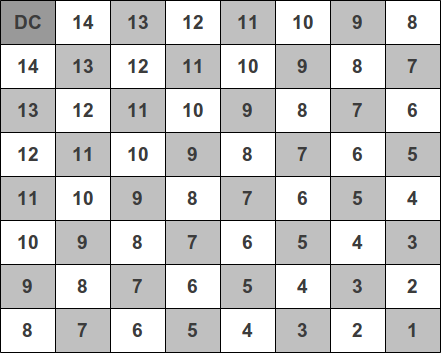
\includegraphics[width=0.5\textwidth]{./imgs/niveisdct.png}
	\caption{Diagonais de energia do bloco DCT.}
	\label{fig:niveisdct}
	\fonte{Autoria própria.}
\end{figure}

O arquivo gerado deve ter as mesmas características do original: tamanho em bytes, largura e altura.

Como exemplo de utilização temos que na execução do comando a seguir, o arquivo saida.yuv de dimensões 352x288 será gerado. O vídeo original será submetido aos valores contidos no arquivo raffle\_352x288.rff e cada janela de dimensões 8x8 terá os níveis DCT (ou diagonais) 1,2,4,6,7,15 zerados.

./block -i entrada.yuv -o saida.yuv -s 352x288 -w 8 -l 1,2,4,6,7,15 -r raffle\_352x288.rff

A única restrição se deve aos valores do arquivo \emph{raffle}, como já mencionado. Este deve conter três colunas, em que a primeira, segunda e terceira colunas devem ter como limites superiores, respectivamente, o número de \emph{frames} do vídeo original e as dimensões largura e altura divididas pelo tamanho da janela (352/8 = 44 e 288/8 = 36).

\subsection{Blur}

A ferramenta blur aplica o artefato de borramento utilizando para tanto um filtro da média ou um filtro da mediana, de dimensão configurável. O arquivo de vídeo de saída é gerado aplicando-se o artefato de acordo com o arquivo \emph{raffle} fornecido por parâmetro. Este, por sua vez, deve conter duas colunas: a primeira indica o \emph{frame} inicial de aplicação, a segunda indica a duração do artefato. Os parâmetros de configuração e respectivas descrições podem ser observados adiante:

\begin{table}[!h]
	\begin{tabular}{llll}
	./blur & & \\ 
	& \texttt{--input} & \texttt{-i}  & arquivo\_de\_entrada \\
	& \texttt{--output} & \texttt{-o}  & arquivo\_de\_saída \\
	& \texttt{--size} & \texttt{-s}  & dimensões do vídeo de entrada no formato WxH \\ 
	& & & (largura por altura em \emph{pixels} ) \\
	& \texttt{--blur} & \texttt{-b}  & tipo do filtro a ser aplicado \\
	& \texttt{--window} & \texttt{-w}  & tamanho do filtro \\
	& \texttt{--rafflelist} & \texttt{-r}  & arquivo\_raffle \\
	& \texttt{--help} & \texttt{-h}  & menu de ajuda \\
	\end{tabular}
\end{table}

Assim como na ferramenta de blocagem, a omissão do parâmetro -r e do arquivo de degradação \emph{raffle} implica na aplicação do borramento em todo o vídeo, de acordo com os parâmetros fornecidos.

Numa possível execução da ferramenta como indicada abaixo, o filtro da média de dimensões 5x5 \emph{pixels} será aplicado no vídeo original, gerando o vídeo degradado saida.yuv de dimensões iguais às do original (\sigla{Full-HD}{Resolução Full-HD de 1080 linhas contendo 1980 \emph{pixels} cada.}).

./blur -i entrada.yuv -o saida.yuv -s 1920x1080 -b average -w 5

Observações:
\begin{itemize}
    \item[-] para utilizar o filtro da média, deve-se fornecer o parâmetro -b \emph{average}, para o filtro da mediana deve-se fornecer o parâmetro -b \emph{median};
    \item[-] a menor dimensão para qualquer tipo de filtro é 3;
\end{itemize}

\subsection{NetSim}

A ferramenta Netsim foi desenvolvida buscando simular degradações ocasionadas pelo processo de decodificação de um streaming de vídeo onde houve perda de informação nas camadas de transporte, rede ou enlace. O Netsim desconsidera, portanto, os artefatos decorrentes do processo de codificação e encapsulamento do vídeo.

As simulações efetuadas pela ferramenta atuam sobre vídeos encapsulados no formato MPEG Transport Stream, conforme definido em \cite{ituh222} e consistem no descarte controlado de porções de informação.

A entidade de dados a ser descartada pode ser tanto um único TS quanto o equivalente a um pacote UDP da camada de transporte, o qual comporta usualmente sete unidades TS.

O descarte é controlado precisamente por meio de um arquivo de configuração fornecido como paramêtro ao programa, podendo este ser gerado pela ferramenta \emph{raffle} descrita em \ref{des:raffle}.

Este arquivo de configuração deve conter duas colunas com valores numéricos inteiros. 

Cada linha será processada sequencialmente, sendo que o primeiro número indica quantas entidades serão transportadas com sucesso e o segundo quantas serão descartadas. 
A Figura \ref{fig:desnetsim} ilustra a sequência.

\begin{figure}[!htb]
	\centering
	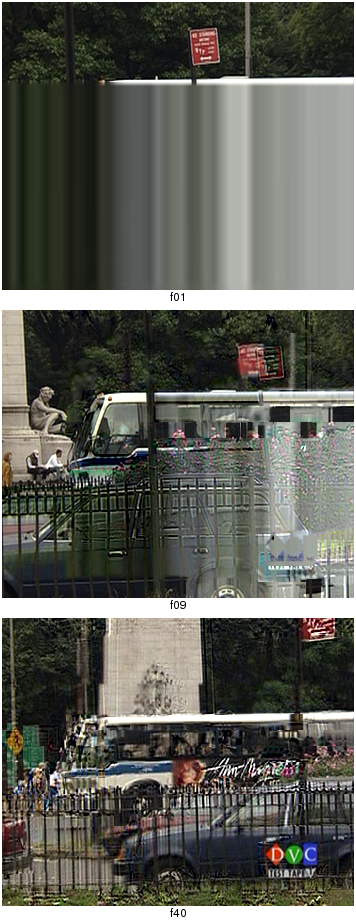
\includegraphics[width=0.9\textwidth]{./imgs/netsim.png}
	\caption{Ilustração do arquivo de configuração de descartes da ferramenta Netsim.}
	\label{fig:desnetsim}
	\fonte{Autoria Própria.}
\end{figure}

Neste caso, \emph{A} e \emph{C} indicam o número de entidades que atingem seu destino com sucesso e \emph{B} e \emph{D} indicam quantas serão descartadas. 
Sendo assim o streaming de vídeo da Figura \ref{fig:netsim}  teria seus primeiros \emph{A} pacotes intactos, seguidos de \emph{B} perdidos, mais \emph{C} pacotes intactos e ainda \emph{D} perdidos novamente.

\begin{table}[!h]
	\begin{tabular}{llll}
	./netsim & & \\
	& \texttt{--input} & \texttt{-i} & Define o caminho (absoluto ou relativo) e arquivo do vídeo \\ 
	& & & a ser processado pela simulação. \\
	& \texttt{--output} & \texttt{-o} & Define o caminho(absoluto ou relativo) e arquivo onde será \\ 
	& & & armazenado o vídeo resultante. \\
	& \texttt{--ts} & \texttt{-t} & (opcional) Se presente, a entidade de descarte considerada \\
	& & & é um TS, caso contrário a unidade é um pacote UDP. \\
	& \texttt{--raffle} & \texttt{-r} & Indica o caminho (absoluto ou relativo) e arquivo a ser usado \\ 
	& & & como configuração de descartes. \\
	\end{tabular}
\end{table}


\subsection{Metric}
\label{des:metric}

A ferramenta Metric se trata da implementação de três métricas objetivas, as mesma encontradas na implementação do SASQV:

\begin{itemize}
	\item MSE
	\item PSNR
	\item MSSIM
\end{itemize}

Implementada em C++, também na forma de uma ferramenta \emph{stand-alone}, seu funcionamento é baseado em verificar disparidades entre dois vídeos fornecidos seguindo uma das métricas implementadas e fornecer um resultado numérico. 
Os vídeos a serem comparados devem possuir as mesmas dimensões e número de \emph{frames} para serem passíveis de comparação. 
A ferramenta Metric pode receber os seguintes parametros:

\begin{table}[!h]
	\begin{tabular}{llll}
	& \texttt{--input} & \texttt{-i} & Define o caminho(absoluto ou relativo) e arquivo onde um dos \\ 
	& & & vídeos a serem comparados se encontra. \\
	& \texttt{--reference} & \texttt{-r} & Define o caminho(absoluto ou relativo) e arquivo onde o segundo \\
	& & & vídeo a ser comparado se encontra. \\
	& \texttt{--size} & \texttt{-s} & Define as dimensões (em \emph{pixels} ) dos vídeos a serem comparados. \\ 
	& & & Deve ser fornecida no formato 'largura'x'altura'. \\
	& \texttt{--metric} & \texttt{-m} & Define qual métrica será utilizada na comparação entre vídeos, \\
	& & & sendo uma string entre MSE, PSNR ou MSSIM. \\
	& \texttt{--window} & \texttt{-w} & Define qual o tamanho da janela (em \emph{pixels} ) a ser usado se \\ 
	& & & a métrica adotada for MSSIM. \\
	\end{tabular}
\end{table}

\section{Interface Gráfica}

A presente seção irá descrever com maiores detalhes as funcionalidades da \emph{interface} gráfica desenvolvida para o SASQV2, separados conforme a finalidade de cada janela presente na mesma.

\subsection{Sessão}

A janela de Sessão possui dois momentos: o de configuração, em que os dados são fornecidos em três telas diferentes; e o de sessão propriamente dita, em que os vídeos são apresentados e avaliados de acordo com a métrica escolhida.

A primeira tela trata de configurações básicas da sessão, tal como um nome e descrição para facilitar a identificação, assim como a métrica que será utilizada e o número de espectadores. Devido as limitações encontradas no \emph{hardware}, somente as métricas DSIS e \sigla{SDSCE}{Simultaneous Double Stimulus for Continuous Evaluation} foram implementadas. As demais, DSCQS e SSCQE, que estão em modo teste no equipamento de avaliação, não foram implementadas pois a modificação do \emph{firmware} não faz parte do escopo deste projeto.

Na sequência é apresentada uma tela em que pode-se buscar e selecionar vídeos para serem exibidos na sessão de avaliação. Por fim, é apresentada a tela para selecionar quais dispositivos remotos serão utilizados na avaliação. Ao final da configuração, pode-se dar início ao processo de avaliação subjetiva onde os vídeos selecionados serão então exibidos.

Na Figura \ref{fig:sessao} pode-se observar o ambiente de exibição dos vídeos durante a avaliação segundo a métrica SDSCE.
Para a execução desta métrica são executados dois players distintos de forma sincronizada, garantindo que ambos exibam o mesmo \emph{frame}.

\begin{figure}[!htb]
	\centering
	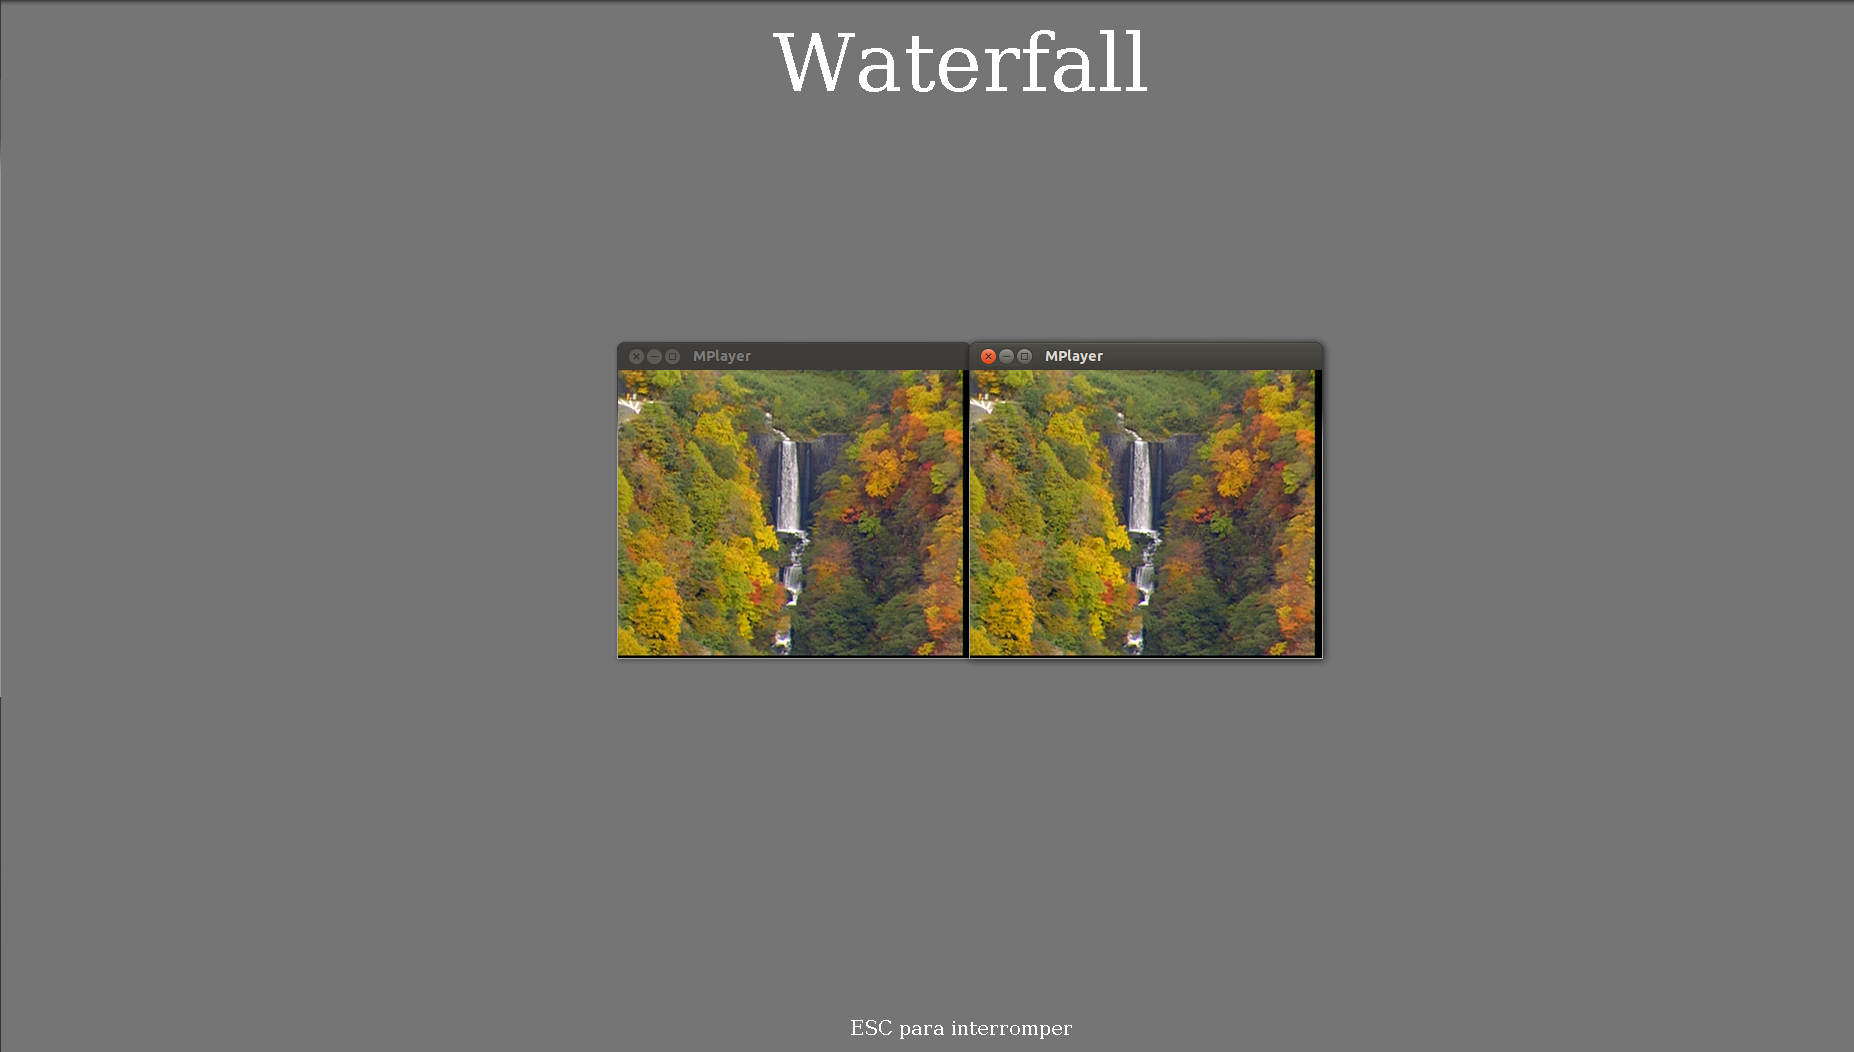
\includegraphics[width=0.9\textwidth]{./imgs/sessao.png}
	\caption{Exemplo de sessão de avaliação.}
	\label{fig:sessao}
	\fonte{Autoria Própria.}
\end{figure}

\subsection{Ferramentas}

Esta é a janela de maior complexidade no SASQV2, dado que nela se encontram os controles e opções que permitem usar todas as ferramentas descritas em \ref{des:ferramentas}. 
Por meio das abas presentes na parte superior da janela é possível acessar três telas diferentes: Gerador de Artefatos, Avaliador Objetivo e Gerador de Aleatoriedade. As funções específicas de cada uma delas são descritas a seguir.

\subsubsection{Gerador de Artefatos}

A tela do gerador de artefatos permite controlar de forma gráfica a execução e parametrização das ferramentas \emph{block}, \emph{blur} e \emph{netsim}. Nela pode-se observar três regiões distintas, presente na figura \ref{fig:geradorartefatos}:

\begin{itemize}
	\item Uma lista de busca dos vídeos passíveis de degradação.
	\item Controladores específicos para cada ferramenta de degradação.
	\item Uma fila de tarefas de degradação a serem executadas.
\end{itemize}

\begin{figure}[!htb]
	\centering
	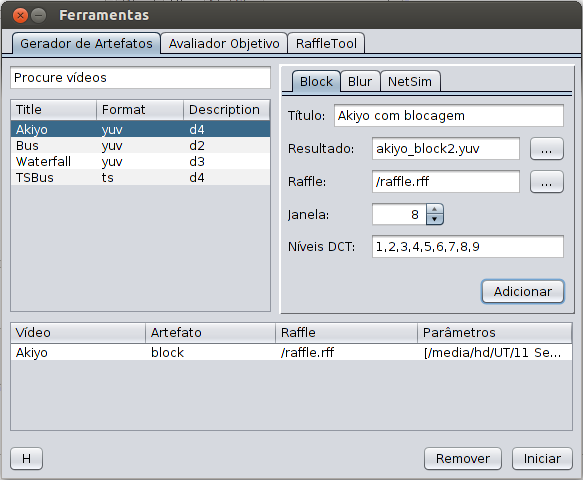
\includegraphics[width=0.9\textwidth]{./imgs/degradacao.png}
	\caption{Janela do gerador de artefatos.}
	\label{fig:geradorartefatos}
	\fonte{Autoria Própria.}
\end{figure}

Para adicionar um artefato em um vídeo é preciso selecionar um vídeo da lista e configurar uma das três ferramentas a disposição. 
Os parâmetros disponíveis na \emph{interface} são condizentes com os parâmetros apresentados em \ref{des:ferramentas} para cada ferramenta.
Ao clicar no botão \emph{Adicionar}, uma tarefa com os detalhes do processo selecionado sera adicionada à lista na parte inferior da tela. É possível enfileirar quantas tarefas forem necessárias e então dar início ao processo de degradação dos vídeos clicando em iniciar.

\subsubsection{Avaliador Objetivo}

Nesta tela existem quatro componentes distintos que permitem configurar e utilizar a ferramenta \emph{metric} citada em \ref{des:metric}:

\begin{itemize}
	\item Uma lista de busca dos vídeos passíveis de avaliação.
	\item Uma lista de busca dos vídeos que podem ser tomados como referência.
	\item Um seletor de métricas objetivas dispiníveis.
	\item Uma fila de tarefas de avaliação a serem executadas.
\end{itemize}

Para efetuar uma avaliação objetiva é preciso selecionar dois vídeos a serem comparados, um como referência e outro como amostra, além da métrica desejada e clicar no botão \emph{Adicionar}.
Com isso, os vídeos e a métrica atualmente selecionados serão adicionados à lista de tarefas. 
Ao se clicar no botão \emph{Iniciar} todas as tarefas da lista serão processadas e uma janela de diálogo mostrará o valor resultante de cada avaliação, os quais também podem ser observados na janela de resultados descrita em \ref{des:resultados}.

\subsubsection{Gerador de Aleatoriedade}

Aqui é possível configurar e utilizar a ferramenta \emph{raffle} de \ref{des:raffle} por meio dos seguintes campos apresentados:

\begin{itemize}
	\item Nome do arquivo a ser gerado.
	\item Número de elementos a serem gerados.
	\item Quantidade de colunas no arquivo de saída.
	\item Tabela de configuração de distribuições estatísticas.
\end{itemize}

Na tabela de configuração, a primeira linha tem o propósito especial de determinar a duração dos artefatos gerados segundo uma distribuição probabilística a ser especificada.
As linhas seguintes permitem a configuração das distribuições utilizadas nas \emph{n} colunas presentes no arquivo.
Os parâmetros de configuração são exatamente os mesmos fornecidos à ferramenta \emph{raffle} em \ref{des:raffle}

\subsection{Resultados}

A janela de resultados é responsável pela visualização e comparação visual dos resultados obtidos por meio de métricas objetivas ou subjetivas.
Nesta tela pode se selecionar um entre dois métodos de visualização: resultados por sessão e resultados por vídeo referência.
No primeiro, o sistema reúne todas as notas subjetivas de uma determinada sessão e as exibe na forma de um gráfico de barras, onde cada barra representa um vídeo, indicando o valor da média e desvio padrão.
Já o segundo exibe um gráfico de pontos, onde o eixo das abscissas apresenta valores referentes à métrica objetiva e o eixo das ordenadas à métrica subjetiva, sendo que cada ponto representa um vídeo degradado a partir de um mesmo vídeo referência.

\label{des:resultados}

\subsection{Configurações}

Esta janela tem o simples propósito de permitir configurar alguns aspectos do sistema SASQV2, tais como os diretórios padrão e os intervalos usados nas fases de apresentação durante a avaliação subjetiva.

\subsection{Ajuda}

A tela de ajuda consiste de uma ampla área de texto dedicada à exibição de páginas \sigla{HTML}{HyperText Markup Language}, na qual foram confeccionados os documentos de ajuda.
Esta janela conta ainda com uma estrutura de navegação topificada no canto esquerdo, proporcionando o acesso direto a uma determinada seção.

\section{Considerações}

A escolha pelo desenvolvimento de ferramentas e módulos independentes na fase de projeto mostrou sua eficiência ao longo do desenvolvimento. 
A primeira vantagem foi vista na efetivação da fase de \emph{design} de código para cada ferramenta em paralelo, divididas entre os membros do projeto.
Essa mesma característica foi vista também durante o desenvolvimento, onde os integrantes podiam trabalhar de forma distribuída.
Contando também com a ferramenta \emph{git} e o repositório \emph{Github} foi possível definir metas semanais de desenvolvimento e integração, minimizando a necessidade de reuniões, as quais foram realizadas usualmente no horário de aula e aos fins de semana.


%---------- Quinto Capítulo: Resultados ----------

\chapter{Resultados} %5 --- 10 pags

Com o conjunto de ferramentas desenvolvidos neste projeto aliado a uma base de vídeos originais é possível produzir e avaliar uma nova e diversificada base com vídeos degradados em qualidade e quantitade variável.
Neste Capítulo serão verificados os resultados obtidos a partir do processamento de vídeos efuados por estas ferramentas. Primeiramente uma avaliação subjetiva das ferramentas de degradação utilizando diversas amostras retiradas de um vídeo da base. A seguir é feita a validação dos resultados obtidos pela ferramenta de métricas objetivas, tomando como base os videos obtidos em \cite{videolab}.
Por fim é feita uma análise das notas de avaliação objetivas buscando mensurar o impacto que determinadas degradações podem ter sobre um conjunto de vídeos com características diferentes.

\section{Validação das Ferramentas de Artefatos}

Foram efetuados diversos processos de degradação sobre o vídeo bus, obtido em \cite{tracevideoseq},  empregando diferentes paramêtros a cada processamento e para cada ferramenta, buscando identificar visualmente e os artefatos produzidos e determinar sua semelhanca com os vistos em situações reais.

A primeira ferramenta a ser avaliada é a \emph{block}.
Para a avaliação foram gerados 14 vídeos onde é efetuado o processo de blocagem, com blocos 8x8, de forma integral --- para todos os blocos em todos os quadros. A cada novo vídeo gerado foram eliminadas de forma cumulativa diagonais na matriz resultante da transformação DCT, partindo da diagonal mais inferior, até que no último vídeo restasse somente a componente DC da transformada. 
Na Figura \ref{fig:blockbus} são apresentados recortes de 160 por 160 \emph{pixels} a partir da posição 64x160 retirados do \emph{frame} de número 60 de cada um dos 14 vídeos obtidos, sendo que o primeiro recorte foi obtido do vídeo original.

Observando os recortes com cautela é possível notar degradações extremamente sutis a partir do recorte \emph{07}, verificadas com mais facilidade nos arredores da publicidade na lateral do ônibus.No recorte de número \emph{10} as regiões de alta frequência da imagem denunciam degradações mais acentuadas, e no \emph{11} já não é mais possível identificar o que está escrito na placa de publicidade, embora ainda seja razoavél identificar a cena da imagem.
Nos três recortes seguintes o efeito de blocagem passa a tomar conta da imagem e apenas objetos de grande escala passam a ser identificáveis, sendo que no recorte de número \emph{14} até mesmo a identificação da cena fica prejudicada.

\begin{figure}[!htb]
	\centering
	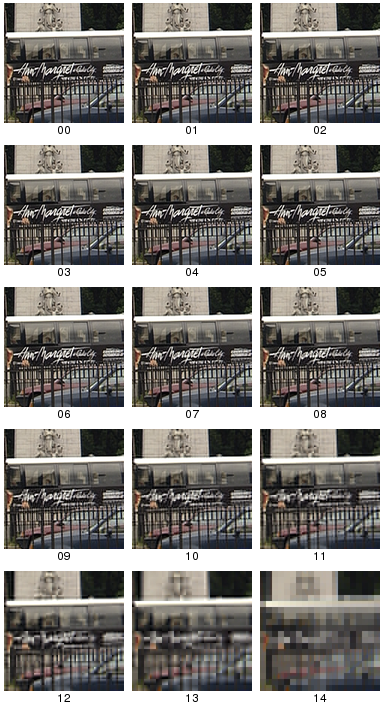
\includegraphics[width=0.8\textwidth]{./imgs/blockbus.png}
	\caption{Sequência de degradações eliminando gradativamente diagonais da DCT.}
	\label{fig:blockbus}
	\fonte{Autoria Própria.}
\end{figure}

Para a avaliação da ferramenta \emph{blur} foram feitas duas sequências de testes, a primeira delas utilizando o filtro de médias e a segunda utilizando o filtro da mediana.
Em cada um dos testes foram utilizadas máscaras matriciais de tamanhos 3x3, 5x5 e 7x7. Nas Figuras \ref{fig:bluraverage} e \ref{fig:blurmedian} são apresentados recortes de 160 por 160 \emph{pixels} a partir da posição 64x160 retirados do \emph{frame} número 60 de cada vídeo.

\begin{figure}[!htb]
	\centering
	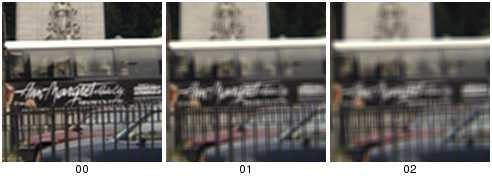
\includegraphics[width=0.9\textwidth]{./imgs/bluraverage.png}
	\caption[Sequência de borramentos aplicando filtro da média]{Sequência de borramentos aplicando filtro da média com matrizes (00) 3x3, (01) 5x5, (02) 7x7.}
	\label{fig:bluraverage}
	\fonte{Autoria Própria.}
\end{figure}

\begin{figure}[!htb]
	\centering
	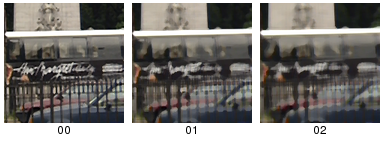
\includegraphics[width=0.9\textwidth]{./imgs/blurmedian.png}
	\caption[Sequência de borramentos aplicando filtro da mediana]{Sequência de borramentos aplicando filtro da mediana com matrizes (00) 3x3, (01) 5x5, (02) 7x7.}
	\label{fig:blurmedian}
	\fonte{Autoria Própria.}
\end{figure}

Na validação visual da ferramenta \emph{raffle} foi gerado um arquivo de sorteio contendo 5 mil elementos.
A distribuição no tempo foi configurada como triangular no intervalo de 0 a 10 com pico no \emph{frame} 5, sendo que a duração de cada artefato foi distribuída uniformemente no intervalo de 1 a 3 \emph{frames}.
Já a distribuição no espaço foi uniforme em toda a largura e altura do \emph{frame}. 
A Figura \ref{fig:busraffle} mostra a sequência de recortes retirados dos 11 \emph{frames} contendo blocos gerados a partir do arquivo raffle obtido com a configuração acima, onde para facilitar a visualização foi eliminada a componente DC da DCT para cada bloco sorteado.

\begin{figure}[!htb]
	\centering
	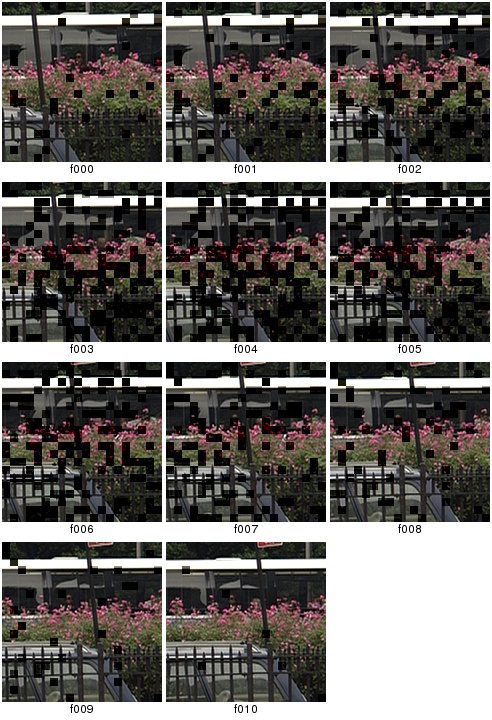
\includegraphics[width=0.8\textwidth]{./imgs/busraffle.png}
	\caption[Sequência de \emph{frames} degradados]{Sequência de \emph{frames} degradados a partir de um arquivo gerado pela ferramenta \emph{raffle}.}
	\label{fig:busraffle}
	\fonte{Autoria Própria.}
\end{figure}

Para o processo de validação da ferramenta \emph{netsim} foi necessário obter um vídeo encapsulado em um TS, para isso foi utilizada a ferramenta ffmpeg para converter o vídeo bus para a codificação MPEG-2 encapsulado em um TS com o seguinte comando:

{
	\centering
	\texttt{ffmpeg -i \emph{arquivo\_de\_entrada} -s cif -sameq -f mpegts -vcodec mpeg2video \emph{arquivo\_de\_saída}}
}

O TS resultante foi então processado pela ferramenta, configurada para fazer os seguintes descartes:

\begin{center}
	\texttt{10 100
	1000 10
	100 10
	1 10
	100 50}
\end{center}

A figura \ref{fig:netsim} contém amostras retiradas dos \emph{frames} 1, 9 e 40, onde podem ser verificados artefatos como \emph{jerkiness}, \emph{blocking} e \emph{bleeding}.

\begin{figure}[!htb]
	\centering
	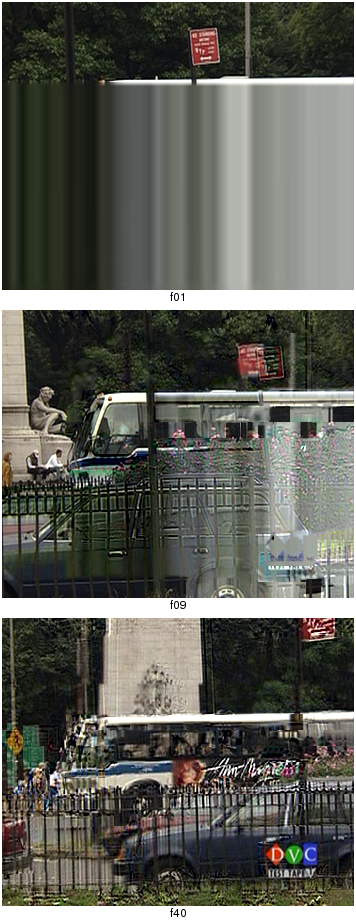
\includegraphics[height=0.9\textheight]{./imgs/netsimresult.png}
	\caption{Amostra de artefados obtidos com a ferramenta \emph{netsim}}
	\label{fig:netsim}
	\fonte{Autoria Própria.}
\end{figure}

\section{Validação da Ferramenta de Métricas}

Para validação dos valores de MSE, PSNR e MSSIM calculados pela ferramenta \emph{metric} foi feita a comparação destes com os obtidos pela ferramenta MSU \emph{Video Quality Measurement Tool}.
%TODO base de videos das metricas
Foram utilizados 5 vídeos diferentes, e os respectivos vídeos degradados,  obtidos em \cite{videolab}. Os resultados das comparações se encontram nas tabelas \ref{res:mse}, \ref{res:psnr} e \ref{res:mssim}.

\begin{table}[!htb]
	\centering
	\caption{Comparação dos resultados de PSNR.}
	\label{res:psnr}
	\begin{tabular}{lccc}
		\hline
		Video	 & MSU	 & SASQV2	 & Erro (\%) \\ \hline
		aircraft	 & 23.49501 & 23.49501 & 0.00000	 \\ 
		liberty	 & 29.21472 & 29.21472 & 0.00000	 \\ 
		ship	 & 25.56667 & 25.56667 & 0.00000	 \\ 
		stockholm & 18.90942 & 18.90942 & 0.00000	 \\ 
		whale	 & 20.59830 & 20.59830 & 0.00000	 \\
	\hline
	\end{tabular}
	\fonte{Autoria pŕopria}
\end{table}

\begin{table}[!htb]
	\centering
	\caption{Comparação dos resultados de MSE.}
	\label{res:mse}
	\begin{tabular}{lccc}
	\hline
	Video	 & MSU	 & SASQV2	 & Erro (\%) \\ \hline
	aircraft	 & 290.78970 & 290.78970 & 0.00000	 \\ 
	liberty	 & 77.91273	 & 77.91273	 & 0.00000	 \\ 
	ship	 & 180.47363 & 180.47362 & -0.00001 \\ 
	stockholm & 835.86987 & 835.86987 & 0.00000	 \\ 
	whale	 & 566.53094 & 566.56611 & 0.00621	 \\
	\hline
	\end{tabular}
	\fonte{Autoria própria}
\end{table}

\begin{table}[!htb]
	\centering
	\caption{Comparação dos resultados de MSSIM.}
	\label{res:mssim}
	\begin{tabular}{lccc}
	\hline
	Video	 & MSU	 & SASQV2	 & Erro (\%) \\ \hline
	aircraft	 & 0.79457 & 0.80723 & 1.59306	 \\
	liberty	 & 0.85415 & 0.85627 & 0.24843	 \\
	ship	 & 0.70462 & 0.70628 & 0.23530	 \\ 
	stockholm & 0.42486 & 0.43327 & 1.97948	 \\ 
	whale	 & 0.81918 & 0.82240 & 0.39320	 \\
	\hline
	\end{tabular}
	\fonte{Autoria própria.}
\end{table}

Observando os resultados para MSE e PSNR pode-se dizer que os resultados são fiéis e que a ferramenta se comporta como o esperado.
A respeito do MSSIM é difícil dizer ao certo o motivo da pequena diferença encontrada nos resultados, especialmente pela variedade de parâmetros a serem levados em conta nesta métrica. 
Levando em conta a documentação do MSU sabe-se que este utiliza pesos uniformes para toda a janela de cálculo, mas não se encontrou o tamanho adotado ou o método de escolha das janelas possíveis.
O teste utilizando a ferramenta presente no SASQV2 utiliza janelas 8x8 adotando janelas não sobrepostas.

\section{Análise de Impacto Sobre Métricas Objetivas}



Para este teste foi utilizada a combinação de três distribuições de artefatos geradas pela ferramenta raffle, que foram concatenadas para criar três rajadas de ruídos em um conjunto de vídeos. As configurações adotadas foram as seguintes:

\begin{enumerate}
	\item Distribuição 1
	\begin{itemize}
		\item Duração: uniforme de 1 a 5
		\item Frames: normal com \(\mu = 25\) e \(\sigma = 10\)
		\item largura: uniforme de 1 a 10
		\item altura: uniforme de 20 a 30
	\end{itemize}
	\item Distribuição 2
	\begin{itemize}
		\item Duração: constante em 3
		\item Frames: uniforme de 70 a 100
		\item largura: uniforme de 10 a 40
		\item altura: uniforme de 10 a 20
	\end{itemize}
	\item Distribuição 3
	\begin{itemize}
		\item Duração: uniforme de 3 a 5
		\item Frames: normal com \(\mu = 220\) e \(\sigma = 40\)
		\item largura: uniforme de 1 a 43
		\item altura: normal com \(\mu = 28\) e \(\sigma = 5\)
	\end{itemize}
\end{enumerate}

O número de artefados em cada \emph{frame} obtido a partir desta configuração é apresentado na figura \ref{fig:histogram}.

Esta configuração foi então usada na aplicação de blocagem em três vídeos diferentes: Akiyo, CoastGuard e Foreman, todos possuindo 300 \emph{frames} de duração e obtidos em \cite{xiph}. Estes vídeos foram escolhidos pelas suas características de textura e movimento, possibilitando uma análise variada.

Nas figuras \ref{fig:mse} e \ref{fig:mssim} pode-se acompanhar a evolução das métricas MSE e MSSIM quadro a quadro para os três vídeos degradados. Observando o comportamento das métricas nota-se que, apesar da natureza e da distribuição dos artefatos utilizados ser exatamente a mesma para todos os vídeos, os valores obtidos possuem picos diferentes, embora o comportamento seja semelhante.

Outro fato notável é a análise individual das métricas, que dependendo do conjunto de \emph{frames} análisado pode levar a conclusões diferentes a respeito do nível de degradação encontrado em cada vídeo.

\begin{figure}[!htb]
	\centering
	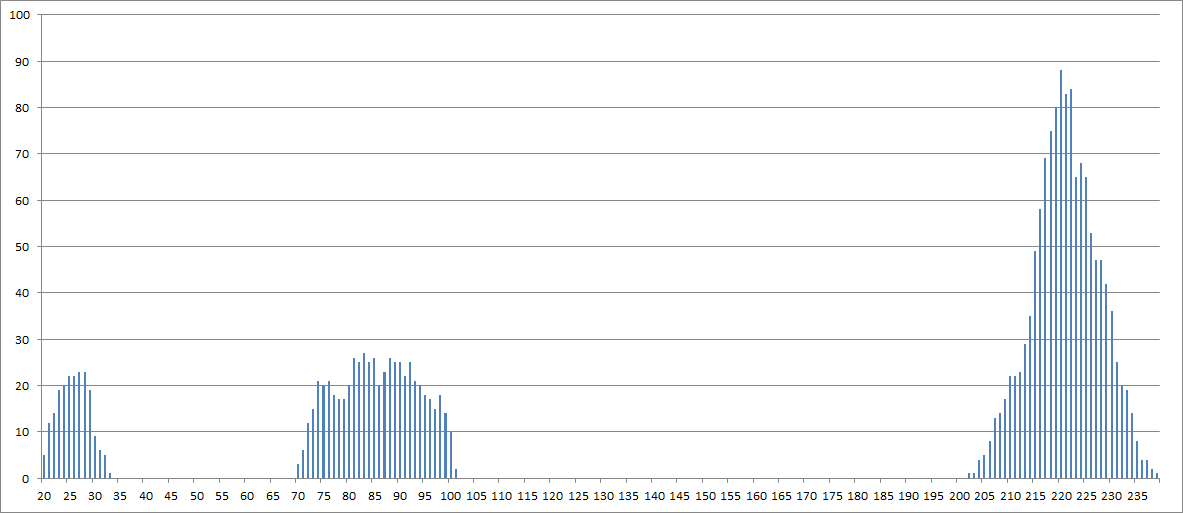
\includegraphics[width=0.9\textwidth]{./imgs/histogram.png}
	\caption{Histograma dos artefatos produzidos}
	\label{fig:histogram}
	\fonte{Autoria Própria.}
\end{figure}

\begin{figure}[!htb]
	\centering
	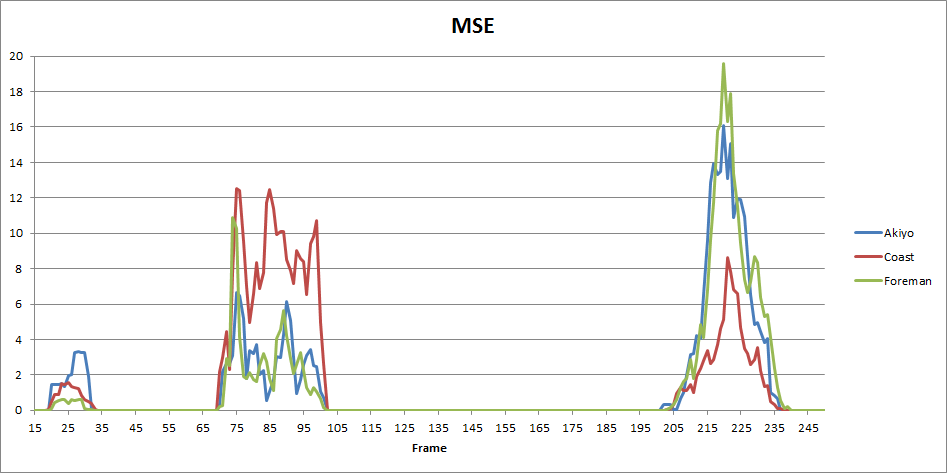
\includegraphics[width=0.9\textwidth]{./imgs/mse.png}
	\caption{MSE quadro a quadro}
	\label{fig:mse}
	\fonte{Autoria Própria.}
\end{figure}

\begin{figure}[!htb]
	\centering
	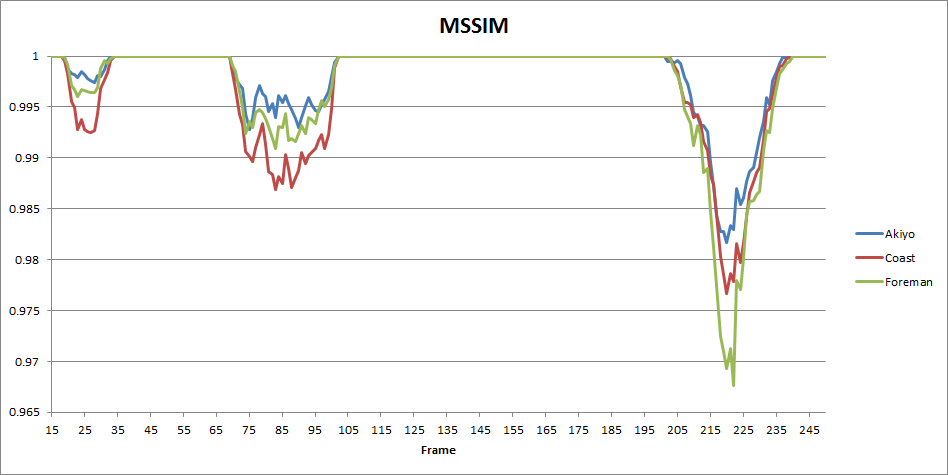
\includegraphics[width=0.9\textwidth]{./imgs/mssim.png}
	\caption{MSSIM quadro a quadro}
	\label{fig:mssim}
	\fonte{Autoria Própria.}
\end{figure}

\section{Resumo e Conclusão do Capítulo}

Neste capítulo foram apresentados resultados visuais proporcionados pelo uso das ferramentas desenvolvidas durante o projeto, demonstrando a flexibilidade e usabilidade do sistema desenvolvido.
Também foram validados os resultados obtidos pelas avaliações objetivas e discutidos aspectos relevantes sobre as possíveis conclusões retiradas a partir dos valores obtidos.


\section{Conclusão}

% ------ estrutura
\subsection{Conclusões}
    \begin{frame}\frametitle{Completude dos Objetivos}
	Quanto às ferramentas:
	\begin{itemize}
		\item Geradores de artefatos
		\begin{itemize}
			\item Configuráveis de forma flexível
			\item Oferecem mais opções
			\item Trabalham sobre arquivos YUV
		\end{itemize}
		\item{Arquivo de degradação}
		\begin{itemize}
			\item Permite reprodução e controle sobre os artefatos
			\item Economia de espaço
		\end{itemize}
		\item Simulador
		\begin{itemize}
			\item Dispensa interfaces físicas
			\item Configurações flexíveis
		\end{itemize}
	\end{itemize}
    \end{frame}

	\begin{frame}\frametitle{Completude dos Objetivos}
	Quanto à Interface:
	\begin{itemize}
		\item Funcionalidades semelhantes ao SASQV
		\item Adaptações para agregar ferramentas e novas utilidades
	\end{itemize}
	Quanto ao sistema:
	\begin{itemize}
		\item Portável, disponível em um arquivo \emph{.jar}
		\item Ferramentas independentes, disponíveis em C++
	\end{itemize}
	\end{frame}
    
\subsection{Trabalhos Futuros}
    \begin{frame}\frametitle{Sugestões}
	\begin{itemize}
		\item extender a funcionalidade do \emph{hardware}
		\item novas ferramentas independentes podem ser criadas
		\item adaptações no BD, agregando mais resultados
		\item aprimoramento da simulação
	\end{itemize}
    \end{frame}
    
\subsection{Fim}
    \begin{frame}\frametitle{Obrigado!}
        \begin{table}[!h]
	        \begin{tabular}{lll}
                Brunno Braga & 41-8898-4111 & brunnobga@gmail.com \\
                Caio Andreatta & 41-8448-7157 & caioccaa@gmail.com \\
	        \end{tabular}
        \end{table}
    \end{frame}



%---------- Referencias ----------
\bibliography{reflatex} % geracao automatica das referencias a partir do arquivo reflatex.bib


%---------- Apendices (opcionais) ----------
%\apendice
%\chapter{Guia de Desenvolvimento}\label{ape:guia} % FIXME: titulo podre
\label{guia}
Este apêndice tem como propósito descrever os passos que podem ser utilizados para obter os arquivos do projeto, reproduzir o ambiente de desenvolvimento, executar o \emph{software} e contribuir com o desenvolvimento do mesmo.
As instruções aqui apresentadas são referentes a uma estação de trabalho utilizando GNU/Linux.
Apesar disso, estas instruções podem também ser utilizadas no sistema operacional Microsoft Windows com poucas modificações.

\section{Obtendo os \emph{Softwares} Necessários}

Para obter, compilar e executar o projeto é necessário que os seguintes \emph{softwares} estejam instalados na estação de trabalho:

\begin{itemize}
% misteriosamente, se eu não colocasse o ~, o texto ficava perto demais do bullet da lista
	\item ~ git, versão 1.7 ou superior.
	\item ~ Java Development Kit 7 ou superior.
	\item ~ Apache Maven, versão 3.0 ou superior.
\end{itemize}

Estes aplicativos podem ser, em geral, obtidos a partir do gerenciador de pacotes da distribuição GNU/Linux.
No caso do Microsoft Windows, é necessário obter estes arquivos a partir da página de cada um dos projetos.

\section{Obtendo os Arquivos do Projeto}

Para obter os arquivos do projeto, basta executar o comando \texttt{clone} do git no repositório do projeto no GitHub:

\lstset{language=bash}
\begin{lstlisting}
git clone git://github.com/onibuscerto/onibuscerto.git
\end{lstlisting}

Ao executar este comando, será criado um diretório \texttt{onibuscerto} com o conteúdo do projeto, conforme a estrutura descrita no Capítulo \ref{chap:desenv}.

\section{Obtendo as Dependências e Compilando o Projeto}

Existem várias formas de se compilar o projeto.
Uma delas, é abrir o projeto em uma IDE que suporte projetos Maven como, por exemplo, a IDE Netbeans.
A outra, é utilizar a ferramenta para linha de comando do próprio Apache Maven.
Para tanto, basta executar o seguinte comando na raiz do diretório \texttt{onibuscerto}:

\lstset{language=bash}
\begin{lstlisting}
mvn install
\end{lstlisting}

Note que este comando irá fazer \emph{download} de todas as dependências do projeto tais como o banco de dados Neo4j, o \emph{framework} de testes JUnit, entre outros.
Sendo assim, o tempo de execução deste comando pode variar de acordo com a velocidade da conexão à Internet sendo utilizada.

Ao concluir o \emph{download} das dependências, o Maven irá automaticamente iniciar a compilação do projeto, após a qual serão executados os testes e o \emph{software} compilado será instalado no repositório local do Maven.
Os testes podem ser executados novamente durante o desenvolvimento a qualquer momento através do comando \texttt{mvn test}.

\section{Importando a Base de Dados}

Duas bases de dados distintas estão presentes no projeto \texttt{onibuscerto-importer}: a primeira, situada no diretório \texttt{onibuscerto-importer/src/test/resources/sample} e apenas utilizada para a execução dos testes, é a base de dados de exemplo da especificação do formato GTFS, a segunda é a base de dados do Bay Area Rapid Transit (BART), da cidade de São Francisco, California.
A base de dados está disponível para uso em \citeonline{bart}.
Para importar a base de dados do BART no banco de dados do \emph{software}, basta executar o seguinte comando a partir do diretório do \texttt{onibuscerto-importer}:

\lstset{language=bash}
\begin{lstlisting}
mvn exec:java -e -Dexec.mainClass="com.onibuscerto.importer.ImporterMain"
\end{lstlisting}

Ao executar este comando, diversas mensagens de depuração serão impressas à saída padrão.
Os arquivos do banco de dados com a base de dados do BART importada serão criados no diretório \texttt{onibuscerto-importer/target/db}.

Após importar a base de dados, é necessário instalar a mesma no projeto \texttt{onibuscerto-service}.
Para tanto, basta copiar o diretório \texttt{onibuscerto-importer/target/db} para o diretório \texttt{onibuscerto-service/target/db}, com o seguinte comando:

\lstset{language=bash}
\begin{lstlisting}
cp -R onibuscerto-importer/target/db onibuscerto-service/target/db
\end{lstlisting}

Ao fim destes passos, o \emph{software} estará devidamente instalado, sendo possível executá-lo com os passos descritos na seção a seguir.

\section{Executando o \emph{Software}}

Para executar o \emph{web service}, basta executar o seguinte comando no diretório \texttt{onibuscerto-service}:

\lstset{language=bash}
\begin{lstlisting}
mvn jetty:run
\end{lstlisting}

Este comando irá automaticamente iniciar uma instância do servidor de aplicações Jetty e instalar o Servlet do projeto no mesmo.
Por fim, o cliente \emph{web} pode ser acessado a partir da URL \texttt{http://localhost:8080/}.
O endereço do \texttt{RouteServlet} será \texttt{http://localhost:8080/route}, sendo que este poderá ser utilizado de acordo com as instruções apresentadas no Apêndice \ref{ape:exemplodeuso}.

%\chapter{Exemplo de Uso do \emph{Service}}\label{ape:exemplodeuso}

Este apêndice procura fornecer um claro exemplo de como executar consultas através do componente \emph{Service} do projeto dentro de uma aplicação.
O código apresentado a seguir, em linguagem Python, executa uma consulta no serviço, decodifica o JSON do objeto resposta e, por fim, imprime o resultado na saída padrão.

Vale lembrar que, para executar este exemplo, é necessário ter instalado o interpretador da linguagem Python na versão 2.6 ou superior.

% TODO: falar que o endereço de acesso do service depende do servidor
% falar também que a URL do RouteServlet depende do especificado no arquivo web.xml do onibuscerto-service/src/main/webapp/WEB-INF

% TODO: será que esse exemplo de cliente em Python fica nessa seção mesmo?
% talvez seja melhor colocar me um anexo ou coisa parecida
% outra coisa, não sei como referenciar ele no texto, então ficou assim msm
\lstinputlisting[language=Python]{code/cliente.py}



% ---------- Anexos (opcionais) ----------
%\anexo
%\chapter{Nome do Anexo}

%Use o comando {\ttfamily \textbackslash anexo} e depois comandos {\ttfamily \textbackslash chapter\{\}}
%para gerar t\'itulos de anexos.


% --------- Lista de siglas --------
%\textbf{* Observa\c{c}\~oes:} a lista de siglas nao realiza a ordenacao das siglas em ordem alfabetica
% Em breve isso sera implementado, enquanto isso:
%\textbf{Sugest\~ao:} crie outro arquivo .tex para siglas e utilize o comando \sigla{sigla}{descri\c{c}\~ao}.
%Para incluir este arquivo no final do arquivo, utilize o comando \input{arquivo.tex}.
%Assim, Todas as siglas serao geradas na ultima pagina. Entao, devera excluir a ultima pagina da versao final do arquivo
% PDF do seu documento.


%-------- Citacoes ---------
% - Utilize o comando \citeonline{...} para citacoes com o seguinte formato: Autor et al. (2011).
% Este tipo de formato eh utilizado no comeco do paragrafo. P.ex.: \citeonline{autor2011}

% - Utilize o comando \cite{...} para citacoeses no meio ou final do paragrafo. P.ex.: \cite{autor2011}



%-------- Titulos com nomes cientificos (titulo, capitulos e secoes) ----------
% Regra para escrita de nomes cientificos:
% Os nomes devem ser escritos em italico, 
%a primeira letra do primeiro nome deve ser em maiusculo e o restante em minusculo (inclusive a primeira letra do segundo nome).
% VEJA os exemplos abaixo.
% 
% 1) voce nao quer que a secao fique com uppercase (caixa alta) automaticamente:
%\section[nouppercase]{\MakeUppercase{Estudo dos efeitos da radiacao ultravioleta C e TFD em celulas de} {\textit{Saccharomyces boulardii}}
%
% 2) por padrao os cases (maiusculas/minuscula) sao ajustados automaticamente, voce nao precisa usar makeuppercase e afins.
% \section{Introducao} % a introducao sera posta no texto como INTRODUCAO, automaticamente, como a norma indica.


\end{document}
